\documentclass[12pt,a4paper, twocolumn]{article}
\usepackage[utf8]{inputenc}
\usepackage{amsmath}
\usepackage[colorlinks]{hyperref}
\hypersetup{
    colorlinks=true,
    linkcolor=blue,
}
\usepackage{amsfonts}
\usepackage{graphicx}
\usepackage{caption}
\usepackage{subcaption}
\usepackage{amssymb}
\usepackage{siunitx}
\DeclareSIUnit\clight{\text{\ensuremath{c}}}
\sisetup{per-mode=symbol}
\usepackage{multicol}
\usepackage{multirow}
\usepackage{fancyhdr}
\usepackage{listings}
\usepackage[switch,columnwise]{lineno}
\usepackage[nottoc]{tocbibind}
\pdfminorversion=6

\pagestyle{fancy}
\fancyhead{} % clear all header fields
\renewcommand{\headrulewidth}{1pt} % no line in header area
\fancyfoot{} % clear all footer fields
\renewcommand{\footrulewidth}{1pt} % no line in header area
\fancyfoot[RE,RO]{\thepage}           % page number in "outer" position of footer line
\newcommand{\Reffig}[1]{Fig.~\ref{#1}}
\newcommand{\Reftbl}[1]{Table.~\ref{#1}}

\usepackage[square,numbers]{natbib}
\bibliographystyle{unsrt}

% def_panda_sym.tex
%
%%%%%%%%%%%%%%%%%%%%%%%%%%%%%%%%%%%%%%%%%%%%%%%%%%%%%%%%%%%%%%%%%%%%%%
%                                                                    %
%  This is pennames.sty                                              %
%                                                                    %
%  It contains the definition of the short names for the PEN         %
%  Elementary Particle Naming Scheme, described in CNL 203, pp 8-11  %
%                                                                    %
%  Version 1.0: Original version -  4 Oct 1991 (evh)                 %
%          1.1: \def,\relax\ifmmode instead of \mbox                 %
%               16 Oct 1991 (mg)                                     %   
%          1.2: Corrections for upsilon and psi - 21 Oct 1991 (evh)  %
%          1.3: Line lenghts < 80 charcaters - 22 Oct 1991 (mg)      %
%          1.4: Add definitions for NFSS (\mathrm instead of \rm)    %
%               27 May 1993 (mg)                                     %   
%          1.5: Add definitions \PaD, \PaDz, \PaB, \PaBz             %
%               \Pq, \Paq, \Pqd, \Paqd, \Pqu, \Paqu, \Pqs, \Paqs     %
%               \Pqc, \Paqc, \Pqb, \Paqb, \Pqt, \Paqt, PaP, PagL     %
%               \PagSm, \PagSp, \PagSz, \PagXz, \PagXp, \PagOp, \PaSq%
%               12 Jul 1993 (mg)                                     %   
%          1.6: Include \relax to force expansion of \if (DCa)       %
%               Add % at end of every command to eliminate possible  %
%               parasitic white space.                               %
%                6 Feb 1994 (mg)                                     %   
%                                                                    %
%  Authors: Michel Goossens and Eric van Herwijnen                   %
%           CERN, Geneva, Switzerland                                %
%                                                                    %
%  Last Mod.  6 Feb 1994 (mg)                                        %
%                                                                    %
%%%%%%%%%%%%%%%%%%%%%%%%%%%%%%%%%%%%%%%%%%%%%%%%%%%%%%%%%%%%%%%%%%%%%%
\ifx\selectfont\undefined% Pre-NFSS font specs
 \def\Pgg{\relax\ifmmode{\rm \gamma}%
          \else${\rm \gamma}$\fi}%
 \def\PW{\relax\ifmmode{\rm W}%
         \else${\rm W }$\fi}%
 \def\PWp{\relax\ifmmode{\rm W^+}%
          \else${\rm W^+}$\fi}%
 \def\PWm{\relax\ifmmode{\rm W^-}%
          \else${\rm W^-}$\fi}%
 \def\PZz{\relax\ifmmode{\rm Z^0}%
          \else${\rm Z^0}$\fi}%
 \def\PHz{\relax\ifmmode{\rm H^0}%
          \else${\rm H^0}$\fi}%
 \def\PHpm{\relax\ifmmode{\rm H^{\pm}}%
           \else${\rm H^{\pm}}$\fi}%
 \def\PWR{\relax\ifmmode{\rm W_R}%
          \else${\rm W_R}$\fi}%
 \def\PWpr{\relax\ifmmode{\rm W^{\prime}}%
           \else${\rm W^{\prime}}$\fi}%
 \def\PZLR{\relax\ifmmode{\rm Z_{LR}}%
           \else${\rm Z_{LR}}$\fi}%
 \def\PZgc{\relax\ifmmode{\rm Z_{\chi}}%
           \else${\rm Z_{\chi}}$\fi}%
 \def\PZgy{\relax\ifmmode{\rm Z_{\psi}}%
           \else${\rm Z_{\psi}}$\fi}%
 \def\PZge{\relax\ifmmode{\rm Z_{\eta}}%
           \else${\rm Z_{\eta}}$\fi}%
 \def\PZi{\relax\ifmmode{\rm Z_1}%
          \else${\rm Z_1}$\fi}%
 \def\PAz{\relax\ifmmode{\rm A^0}%
          \else${\rm A^0}$\fi}%
 \def\Pgne{\relax\ifmmode{\nu_{\rm e}}%
           \else$\nu_{\rm e}$\fi}%
 \def\Pagne{\relax\ifmmode{\overline{\nu}_{\rm e}}%
            \else$\overline{\nu}_{\rm e}$\fi}%
 \def\Pgngm{\relax\ifmmode{\rm \nu_{\mu}}%
            \else${\rm \nu_{\mu}}$\fi}%
 \def\Pagngm{\relax\ifmmode{\rm \overline{\nu}_{\mu}}%
             \else${\rm \overline{\nu}_{\mu}}$\fi}%
 \def\Pgngt{\relax\ifmmode{\rm \nu_{\tau}}%
            \else${\rm \nu_{\tau}}$\fi}%
 \def\Pagngt{\relax\ifmmode{\rm \overline{\nu}_{\tau}}%
             \else${\rm \overline{\nu}_{\tau}}$\fi}%
 \def\Pe{\relax\ifmmode{\rm e}%
         \else${\rm e}$\fi}%
 \def\Pep{\relax\ifmmode{\rm e^+}%
          \else${\rm e^+}$\fi}%
 \def\Pem{\relax\ifmmode{\rm e^-}%
          \else${\rm e^-}$\fi}%
 \def\Pepm{\relax\ifmmode{\rm e^\pm}%
          \else${\rm e^\pm}$\fi}%
 \def\Pgm{\relax\ifmmode{\rm \mu}%
          \else${\rm \mu}$\fi}%
 \def\Pgmm{\relax\ifmmode{\rm \mu^-}%
           \else${\rm \mu^-}$\fi}%
 \def\Pgmp{\relax\ifmmode{\rm \mu^+}%
           \else${\rm \mu^+}$\fi}%
 \def\Pgmpm{\relax\ifmmode{\rm \mu^\pm}%
           \else${\rm \mu^\pm}$\fi}%
 \def\Pgt{\relax\ifmmode{\rm \tau}%
          \else${\rm \tau}$\fi}%
 \def\PLpm{\relax\ifmmode{\rm L^{\pm}}%
           \else${\rm L^{\pm}}$\fi}%
 \def\PLz{\relax\ifmmode{\rm L^0}%
          \else${\rm L^0}$\fi}%
 \def\PEz{\relax\ifmmode{\rm E^0}%
          \else${\rm E^0}$\fi}%
 \def\Pgp{\relax\ifmmode{\rm \pi}%
          \else${\rm \pi }$\fi}%
 \def\Pgpm{\relax\ifmmode{\rm \pi^-}%
           \else${\rm \pi^-}$\fi}%
 \def\Pgpp{\relax\ifmmode{\rm \pi^+}%
           \else${\rm \pi^+}$\fi}%
 \def\Pgppm{\relax\ifmmode{\rm \pi^{\pm }}%
            \else${\rm \pi^{\pm }}$\fi}%
 \def\Pgpz{\relax\ifmmode{\rm \pi^0}%
           \else${\rm \pi^0 }$\fi}%
 \def\Pgh{\relax\ifmmode{\rm \eta}%
          \else${\rm \eta }$\fi}%
 \def\Pgr{\relax\ifmmode{\rm \rho(770)}%
          \else${\rm \rho(770)}$\fi}%
 \def\Pgo{\relax\ifmmode{\rm \omega(783)}%
          \else${\rm \omega(783)}$\fi}%
 \def\Pghpr{\relax\ifmmode{\rm \eta^{\prime}(958)}%
            \else${\rm \eta^{\prime}(958)}$\fi}%
 \def\Pfz{\relax\ifmmode{\rm f_0(975)}%
          \else${\rm f_0(975)}$\fi}%
 \def\Paz{\relax\ifmmode{\rm a_0(980)}%
          \else${\rm a_0(980)}$\fi}%
 \def\Pgf{\relax\ifmmode{\rm \phi(1020)}%
          \else${\rm \phi(1020)}$\fi}%
 \def\Phia{\relax\ifmmode{\rm h_1(1170)}%
           \else${\rm h_1(1170)}$\fi}%
 \def\Pbi{\relax\ifmmode{\rm b_1(1235)}%
          \else${\rm b_1(1235)}$\fi}%
 \def\Pai{\relax\ifmmode{\rm a_1(1260)}%
          \else${\rm a_1(1260)}$\fi}%
 \def\Pfii{\relax\ifmmode{\rm f_2(1270)}%
           \else${\rm f_2(1270)}$\fi}%
 \def\Pfi{\relax\ifmmode{\rm f_1(1285)}%
          \else${\rm f_1(1285)}$\fi}%
 \def\Pgha{\relax\ifmmode{\rm \eta(1295)}%
           \else${\rm \eta(1295)}$\fi}%
 \def\Pgpa{\relax\ifmmode{\rm \pi(1300)}%
           \else${\rm \pi(1300)}$\fi}%
 \def\Paii{\relax\ifmmode{\rm a_2(1320)}%
           \else${\rm a_2(1320)}$\fi}%
 \def\Pgoa{\relax\ifmmode{\rm \omega(1390)}%
           \else${\rm \omega(1390)}$\fi}%
 \def\Pfza{\relax\ifmmode{\rm f_0(1400)}%
           \else${\rm f_0(1400)}$\fi}%
 \def\Pfia{\relax\ifmmode{\rm f_1 (1390)}%
           \else${\rm f_1 (1390)}$\fi}%
 \def\Pghb{\relax\ifmmode{\rm \eta(1440)}%
           \else${\rm \eta(1440)}$\fi}%
 \def\Pgra{\relax\ifmmode{\rm \rho(1450)}%
           \else${\rm \rho(1450)}$\fi}%
 \def\Pfib{\relax\ifmmode{\rm f_1(1510)}%
           \else${\rm f_1(1510)}$\fi}%
 \def\Pfiipr{\relax\ifmmode{\rm f^{\prime}_2(1525)}%
             \else${\rm f^{\prime}_2(1525)}$\fi}%
 \def\Pfzb{\relax\ifmmode{\rm f_0(1590)}%
           \else${\rm f_0(1590)}$\fi}%
 \def\Pgob{\relax\ifmmode{\rm \omega(1600)}%
           \else${\rm \omega(1600)}$\fi}%
 \def\Pgoiii{\relax\ifmmode{\rm \omega_3(1670)}%
             \else${\rm \omega_3(1670)}$\fi}%
 \def\Pgpii{\relax\ifmmode{\rm \pi_2(1670)}%
            \else${\rm \pi_2(1670)}$\fi}%
 \def\Pgfa{\relax\ifmmode{\rm \phi(1680)}%
           \else${\rm \phi(1680)}$\fi}%
 \def\Pgriii{\relax\ifmmode{\rm \rho_3(1690)}%
             \else${\rm \rho_3(1690)}$\fi}%
 \def\Pgrb{\relax\ifmmode{\rm \rho(1700)}%
           \else${\rm \rho(1700)}$\fi}%
 \def\Pfiia{\relax\ifmmode{\rm f_2(1720)}%
            \else${\rm f_2(1720)}$\fi}%
 \def\Pgfiii{\relax\ifmmode{\rm \phi_3(1850)}%
             \else${\rm \phi_3(1850)}$\fi}%
 \def\Pfiib{\relax\ifmmode{\rm f_2(2010)}%
            \else${\rm f_2(2010)}$\fi}%
 \def\Pfiv{\relax\ifmmode{\rm f_4(2050)}%
           \else${\rm f_4(2050)}$\fi}%
 \def\Pfiic{\relax\ifmmode{\rm f_2(2300)}%
            \else${\rm f_2(2300)}$\fi}%
 \def\Pfiid{\relax\ifmmode{\rm f_2(2340)}%
            \else${\rm f_2(2340)}$\fi}%
 \def\PK{\relax\ifmmode{\rm K}%
         \else${\rm K}$\fi}%
 \def\PKpm{\relax\ifmmode{\rm K^{\pm}}%
           \else${\rm K^{\pm}}$\fi}%
 \def\PKp{\relax\ifmmode{\rm K^+}%
          \else${\rm K^+}$\fi}%
 \def\PKm{\relax\ifmmode{\rm K^-}%
          \else${\rm K^-}$\fi}%
 \def\PKz{\relax\ifmmode{\rm K^0}%
          \else${\rm K^0}$\fi}%
 \def\PaKz{\relax\ifmmode{\overline{\rm K}^0}%
           \else$\overline{\rm K}^0$\fi}%
 \def\PKgmiii{\relax\ifmmode{\rm K_{\mu 3}}%
              \else${\rm K_{\mu 3}}$\fi}%
 \def\PKeiii{\relax\ifmmode{\rm K_{\rm e3}}%
             \else${\rm K_{\rm e3}}$\fi}%
 \def\PKzS{\relax\ifmmode{\rm K^0_{\rm S}}%
           \else${\rm K^0_{\rm S}}$\fi}%
 \def\PKzL{\relax\ifmmode{\rm K^0_{\rm L}}%
           \else${\rm K^0_{\rm L}}$\fi}%
 \def\PKzgmiii{\relax\ifmmode{\rm K^0_{\mu 3}}%
               \else${\rm K^0_{\mu 3}}$\fi}%
 \def\PKzeiii{\relax\ifmmode{\rm K^0_{{\rm e}3}}%
              \else${\rm K^0_{{\rm e}3}}$\fi}%
 \def\PKst{\relax\ifmmode{\rm K^{\ast}(892)}%
           \else${\rm K^{\ast}(892)}$\fi}%
 \def\PKi{\relax\ifmmode{\rm K_1(1270)}%
          \else${\rm K_1(1270)}$\fi}%
 \def\PKsta{\relax\ifmmode{\rm K^{\ast}(1370)}%
            \else${\rm K^{\ast}(1370)}$\fi}%
 \def\PKia{\relax\ifmmode{\rm K_1(1400)}%
           \else${\rm K_1(1400)}$\fi}%
 \def\PKstz{\relax\ifmmode{\rm K^{\ast}_0(1430)}%
            \else${\rm K^{\ast}_0(1430)}$\fi}%
 \def\PKstii{\relax\ifmmode{\rm K^{\ast}_2(1430)}%
             \else${\rm K^{\ast}_2(1430)}$\fi}%
 \def\PKstb{\relax\ifmmode{\rm K^{\ast}(1680)}%
            \else${\rm K^{\ast}(1680)}$\fi}%
 \def\PKii{\relax\ifmmode{\rm K_2(1770)}%
           \else${\rm K_2(1770)}$\fi}%
 \def\PKstiii{\relax\ifmmode{\rm K^{\ast}_3(1780)}%
              \else${\rm K^{\ast}_3(1780)}$\fi}%
 \def\PKstiv{\relax\ifmmode{\rm K^{\ast}_4(2045)}%
             \else${\rm K^{\ast}_4(2045)}$\fi}%
 \def\PD{\relax\ifmmode{\rm D}%
           \else${\rm D}$\fi}%
 \def\PaD{\relax\ifmmode{\rm \overline{D}}%
           \else${\rm \overline{D}}$\fi}%
 \def\PDpm{\relax\ifmmode{\rm D^{\pm}}%
           \else${\rm D^{\pm}}$\fi}%
 \def\PDm{\relax\ifmmode{\rm D^-}%
          \else${\rm D^-}$\fi}%
 \def\PDp{\relax\ifmmode{\rm D^+}%
          \else${\rm D^+}$\fi}%
 \def\PDz{\relax\ifmmode{\rm D^0}%
          \else${\rm D^0}$\fi}%
 \def\PaDz{\relax\ifmmode{\overline{\rm D}^0}%
           \else$\overline{\rm D}^0$\fi}%
 \def\PDstpm{\relax\ifmmode{{\rm D}^{\ast}(2010)^{\pm}}%
             \else${\rm D}^{\ast}(2010)^{\pm}$\fi}%
 \def\PDstz{\relax\ifmmode{{\rm D}^{\ast}(2010)^0}%
            \else${\rm D}^{\ast}(2010)^0$\fi}%
 \def\PDiz{\relax\ifmmode{{\rm D}_{1}(2420)^0}%
           \else${\rm D}_{1}(2420)^0$\fi}%
 \def\PDstiiz{\relax\ifmmode{{\rm D}^{\ast}_{2}(2460)^0}%
              \else${\rm D}^{\ast}_{2}(2460)^0$\fi}%
 \def\PsDp{\relax\ifmmode{\rm D_{s}^+}%
           \else${\rm D_{s}^+}$\fi}%
 \def\PsDm{\relax\ifmmode{\rm D_{s}^-}%
           \else${\rm D_{s}^-}$\fi}%
 \def\PsDst{\relax\ifmmode{\rm D_{s}^{\ast}}%
            \else${\rm D_{s}^{\ast}}$\fi}%
 \def\PsDipm{\relax\ifmmode{\rm D_{s1}(2536)^{\pm}}%
           \else${\rm D_{s1}(2536)^{\pm}}$\fi}%
 \def\PB{\relax\ifmmode{{\rm B}}%
          \else${\rm B}$\fi}%
 \def\PaB{\relax\ifmmode{{\rm \overline{B}}}%
          \else${\rm \overline{B}}$\fi}%
 \def\PBp{\relax\ifmmode{{\rm B}^{+}}%
           \else${\rm B}^{+}$\fi}%
 \def\PBm{\relax\ifmmode{{\rm B}^{-}}%
           \else${\rm B}^{-}$\fi}%
 \def\PBpm{\relax\ifmmode{{\rm B}^{\pm}}%
            \else${\rm B}^{\pm}$\fi}%
 \def\PBz{\relax\ifmmode{{\rm B}^0}%
           \else${\rm B}^0$\fi}%
 \def\PaBz{\relax\ifmmode{{\rm \overline{B}}^0}%
           \else${\rm \overline{B}}^0$\fi}%
 \def\Pcgh{\relax\ifmmode{\rm {\eta}_{c}(1S)}%
           \else${\rm {\eta}_{c}(1S)}$\fi}%
 \def\PJgy{\relax\ifmmode{\rm J /\psi(1S)}%
           \else${\rm J /\psi(1S)}$\fi}%
 \def\Pcgcz{\relax\ifmmode{\rm {\chi}_{c0}(1P)}%
            \else${\rm {\chi}_{c0}(1P)}$\fi}%
 \def\Pcgci{\relax\ifmmode{\rm {\chi}_{c1}(1P)}%
            \else${\rm {\chi}_{c1}(1P)}$\fi}%
 \def\Pcgcii{\relax\ifmmode{\rm {\chi}_{c2}(1P)}%
             \else${\rm {\chi}_{c2}(1P)}$\fi}%
 \def\Pgy{\relax\ifmmode{\rm \psi(2S)}%
          \else${\rm \psi(2S)}$\fi}%
 \def\Pgya{\relax\ifmmode{\rm \psi(3770)}%
           \else${\rm \psi(3770)}$\fi}%
 \def\Pgyb{\relax\ifmmode{\rm \psi(4040)}%
           \else${\rm \psi(4040)}$\fi}%
 \def\Pgyc{\relax\ifmmode{\rm \psi(4160)}%
           \else${\rm \psi(4160)}$\fi}%
 \def\Pgyd{\relax\ifmmode{\rm \psi(4415)}%
           \else${\rm \psi(4415)}$\fi}%
 \def\PgU{\relax\ifmmode{\rm \Upsilon(1S)}%
          \else${\rm \Upsilon(1S)}$\fi}%
 \def\Pbgcz{\relax\ifmmode{\rm {\chi}_{b0}(1P)}%
            \else${\rm {\chi}_{b0}(1P)}$\fi}%
 \def\Pbgci{\relax\ifmmode{\rm {\chi}_{b1}(1P)}%
            \else${\rm {\chi}_{b1}(1P)}$\fi}%
 \def\Pbgcii{\relax\ifmmode{\rm {\chi}_{b2}(1P)}%
             \else${\rm {\chi}_{b2}(1P)}$\fi}%
 \def\PgUa{\relax\ifmmode{\rm \Upsilon(2S)}%
           \else${\rm \Upsilon(2S)}$\fi}%
 \def\Pbgcza{\relax\ifmmode{\rm {\chi}_{b0}(2P)}%
             \else${\rm {\chi}_{b0}(2P)}$\fi}%
 \def\Pbgcia{\relax\ifmmode{\rm {\chi}_{b1}(2P)}%
             \else${\rm {\chi}_{b1}(2P)}$\fi}%
 \def\Pbgciia{\relax\ifmmode{\rm {\chi}_{b2}(2P)}%
              \else${\rm {\chi}_{b2}(2P)}$\fi}%
 \def\PgUb{\relax\ifmmode{\rm \Upsilon(3S)}%
           \else${\rm \Upsilon(3S)}$\fi}%
 \def\PgUc{\relax\ifmmode{\rm \Upsilon(4S)}%
           \else${\rm \Upsilon(4S)}$\fi}%
 \def\PgUd{\relax\ifmmode{\rm \Upsilon(10860)}%
           \else${\rm \Upsilon(10860)}$\fi}%
 \def\PgUe{\relax\ifmmode{\rm \Upsilon(11020)}%
           \else${\rm \Upsilon(11020)}$\fi}%
 \def\Pq{\relax\ifmmode{\rm q}%
         \else${\rm q}$\fi}%
 \def\Paq{\relax\ifmmode{\rm \overline{q}}%
         \else${\rm \overline{q}}$\fi}%
 \def\Pqd{\relax\ifmmode{\rm q_d}%
         \else${\rm q_d}$\fi}%
 \def\Paqd{\relax\ifmmode{\rm \overline{q}_d}%
         \else${\rm \overline{q}_d}$\fi}%
 \def\Pqu{\relax\ifmmode{\rm q_u}%
         \else${\rm q_u}$\fi}%
 \def\Paqu{\relax\ifmmode{\rm \overline{q}_u}%
         \else${\rm \overline{q}_u}$\fi}%
 \def\Pqs{\relax\ifmmode{\rm q_s}%
         \else${\rm q_s}$\fi}%
 \def\Paqs{\relax\ifmmode{\rm \overline{q}_s}%
         \else${\rm \overline{q}_s}$\fi}%
 \def\Pqc{\relax\ifmmode{\rm q_c}%
         \else${\rm q_c}$\fi}%
 \def\Paqc{\relax\ifmmode{\rm \overline{q}_c}%
         \else${\rm \overline{q}_c}$\fi}%
 \def\Pqb{\relax\ifmmode{\rm q_b}%
         \else${\rm q_b}$\fi}%
 \def\Paqb{\relax\ifmmode{\rm \overline{q}_b}%
         \else${\rm \overline{q}_b}$\fi}%
 \def\Pqt{\relax\ifmmode{\rm q_t}%
         \else${\rm q_t}$\fi}%
 \def\Paqt{\relax\ifmmode{\rm \overline{q}_t}%
         \else${\rm \overline{q}_t}$\fi}%
 \def\Pp{\relax\ifmmode{\rm p}%
         \else${\rm p}$\fi}%
 \def\Pap{\relax\ifmmode{\rm \overline{p}}%
         \else${\rm \overline{p}}$\fi}%
 \def\Pn{\relax\ifmmode{\rm n}%
         \else${\rm n}$\fi}%
 \def\PNa{\relax\ifmmode{\rm N(1440)P_{11}}%
          \else${\rm N(1440)P_{11}}$\fi}%
 \def\PNb{\relax\ifmmode{\rm N(1520)D_{13}}%
          \else${\rm N(1520)D_{13}}$\fi}%
 \def\PNc{\relax\ifmmode{\rm N(1535)S_{11}}%
          \else${\rm N(1535)S_{11}}$\fi}%
 \def\PNd{\relax\ifmmode{\rm N(1650)S_{11}}%
          \else${\rm N(1650)S_{11}}$\fi}%
 \def\PNe{\relax\ifmmode{\rm N(1675)D_{15}}%
          \else${\rm N(1675)D_{15}}$\fi}%
 \def\PNf{\relax\ifmmode{\rm N(1680)F_{15}}%
          \else${\rm N(1680)F_{15}}$\fi}%
 \def\PNg{\relax\ifmmode{\rm N(1700)D_{13}}%
          \else${\rm N(1700)D_{13}}$\fi}%
 \def\PNh{\relax\ifmmode{\rm N(1710)P_{11}}%
          \else${\rm N(1710)P_{11}}$\fi}%
 \def\PNi{\relax\ifmmode{\rm N(1720)P_{13}}%
          \else${\rm N(1720)P_{13}}$\fi}%
 \def\PNj{\relax\ifmmode{\rm N(2190)G_{17}}%
          \else${\rm N(2190)G_{17}}$\fi}%
 \def\PNk{\relax\ifmmode{\rm N(2220)H_{19}}%
          \else${\rm N(2220)H_{19}}$\fi}%
 \def\PNl{\relax\ifmmode{\rm N(2250)G_{19}}%
          \else${\rm N(2250)G_{19}}$\fi}%
 \def\PNm{\relax\ifmmode{\rm N(2600)I_{1,11}}%
          \else${\rm N(2600)I_{1,11}}$\fi}%
 \def\PgDa{\relax\ifmmode{\rm \Delta(1232)P_{33}}%
           \else${\rm \Delta(1232)P_{33}}$\fi}%
 \def\PgDb{\relax\ifmmode{\rm \Delta(1620)S_{31}}%
           \else${\rm \Delta(1620)S_{31}}$\fi}%
 \def\PgDc{\relax\ifmmode{\rm \Delta(1700)D_{33}}%
           \else${\rm \Delta(1700)D_{33}}$\fi}%
 \def\PgDd{\relax\ifmmode{\rm \Delta(1900)S_{31}}%
           \else${\rm \Delta(1900)S_{31}}$\fi}%
 \def\PgDe{\relax\ifmmode{\rm \Delta(1905)F_{35}}%
           \else${\rm \Delta(1905)F_{35}}$\fi}%
 \def\PgDf{\relax\ifmmode{\rm \Delta(1910)P_{31}}%
           \else${\rm \Delta(1910)P_{31}}$\fi}%
 \def\PgDh{\relax\ifmmode{\rm \Delta(1920)P_{33}}%
           \else${\rm \Delta(1920)P_{33}}$\fi}%
 \def\PgDi{\relax\ifmmode{\rm \Delta(1930)D_{35}}%
           \else${\rm \Delta(1930)D_{35}}$\fi}%
 \def\PgDj{\relax\ifmmode{\rm \Delta(1950)F_{37}}%
           \else${\rm \Delta(1950)F_{37}}$\fi}%
 \def\PgDk{\relax\ifmmode{\rm \Delta(2420)H_{3,11}}%
           \else${\rm \Delta(2420)H_{3,11}}$\fi}%
 \def\PgL{\relax\ifmmode{\rm \Lambda}%
          \else${\rm \Lambda}$\fi}%
 \def\PagL{\relax\ifmmode{\rm \overline{\Lambda}}%
          \else${\rm \overline{\Lambda}}$\fi}%
 \def\PgLa{\relax\ifmmode{\rm \Lambda(1405) S_{01}}%
           \else${\rm \Lambda(1405) S_{01}}$\fi}%
 \def\PgLb{\relax\ifmmode{\rm \Lambda(1520) D_{03}}%
           \else${\rm \Lambda(1520) D_{03}}$\fi}%
 \def\PgLc{\relax\ifmmode{\rm \Lambda(1600) P_{01}}%
           \else${\rm \Lambda(1600) P_{01}}$\fi}%
 \def\PgLd{\relax\ifmmode{\rm \Lambda(1670) S_{01}}%
           \else${\rm \Lambda(1670) S_{01}}$\fi}%
 \def\PgLe{\relax\ifmmode{\rm \Lambda(1690) D_{03}}%
           \else${\rm \Lambda(1690) D_{03}}$\fi}%
 \def\PgLf{\relax\ifmmode{\rm \Lambda(1800) S_{01}}%
           \else${\rm \Lambda(1800) S_{01}}$\fi}%
 \def\PgLg{\relax\ifmmode{\rm \Lambda(1810) P_{01}}%
           \else${\rm \Lambda(1810) P_{01}}$\fi}%
 \def\PgLh{\relax\ifmmode{\rm \Lambda(1820) F_{05}}%
           \else${\rm \Lambda(1820) F_{05}}$\fi}%
 \def\PgLi{\relax\ifmmode{\rm \Lambda(1830) D_{05}}%
           \else${\rm \Lambda(1830) D_{05}}$\fi}%
 \def\PgLj{\relax\ifmmode{\rm \Lambda(1890) P_{03}}%
           \else${\rm \Lambda(1890) P_{03}}$\fi}%
 \def\PgLk{\relax\ifmmode{\rm \Lambda(2100) G_{07}}%
           \else${\rm \Lambda(2100) G_{07}}$\fi}%
 \def\PgLl{\relax\ifmmode{\rm \Lambda(2110) F_{05}}%
           \else${\rm \Lambda(2110) F_{05}}$\fi}%
 \def\PgLm{\relax\ifmmode{\rm \Lambda(2350) H_{09}}%
           \else${\rm \Lambda(2350) H_{09}}$\fi}%
 \def\PgSp{\relax\ifmmode{\rm \Sigma^+}%
           \else${\rm \Sigma^+}$\fi}%
 \def\PagSp{\relax\ifmmode{\rm \overline{\Sigma}^+}%
           \else${\rm \overline{\Sigma}^+}$\fi}%
 \def\PgSz{\relax\ifmmode{\rm \Sigma^0}%
           \else${\rm \Sigma^0}$\fi}%
 \def\PagSz{\relax\ifmmode{\rm \overline{\Sigma}^0}%
           \else${\rm \overline{\Sigma}^0}$\fi}%
 \def\PgSm{\relax\ifmmode{\rm \Sigma^-}%
           \else${\rm \Sigma^-}$\fi}%
 \def\PagSm{\relax\ifmmode{\rm \overline{\Sigma}^-}%
           \else${\rm \overline{\Sigma}^-}$\fi}%
 \def\PgSa{\relax\ifmmode{\rm \Sigma(1385) P_{13}}%
           \else${\rm \Sigma(1385) P_{13}}$\fi}%
 \def\PgSb{\relax\ifmmode{\rm \Sigma(1660) P_{11}}%
           \else${\rm \Sigma(1660) P_{11}}$\fi}%
 \def\PgSc{\relax\ifmmode{\rm \Sigma(1670) D_{13}}%
           \else${\rm \Sigma(1670) D_{13}}$\fi}%
 \def\PgSd{\relax\ifmmode{\rm \Sigma(1750) S_{11}}%
           \else${\rm \Sigma(1750) S_{11}}$\fi}%
 \def\PgSe{\relax\ifmmode{\rm \Sigma(1775) D_{15}}%
           \else${\rm \Sigma(1775) D_{15}}$\fi}%
 \def\PgSf{\relax\ifmmode{\rm \Sigma(1915) F_{15}}%
           \else${\rm \Sigma(1915) F_{15}}$\fi}%
 \def\PgSg{\relax\ifmmode{\rm \Sigma(1940) D_{13}}%
           \else${\rm \Sigma(1940) D_{13}}$\fi}%
 \def\PgSh{\relax\ifmmode{\rm \Sigma(2030) F_{17}}%
           \else${\rm \Sigma(2030) F_{17}}$\fi}%
 \def\PgSi{\relax\ifmmode{\rm \Sigma(2050)}%
           \else${\rm \Sigma(2050)}$\fi}%
 \def\PgXz{\relax\ifmmode{\rm \Xi^0}%
           \else${\rm \Xi^0}$\fi}%
 \def\PagXz{\relax\ifmmode{\rm \overline{\Xi}^0}%
           \else${\rm \overline{\Xi}^0}$\fi}%
 \def\PgXm{\relax\ifmmode{\rm \Xi^-}%
           \else${\rm \Xi^-}$\fi}%
 \def\PagXp{\relax\ifmmode{\rm \overline{\Xi}^+}%
           \else${\rm \overline{\Xi}^+}$\fi}%
 \def\PgXa{\relax\ifmmode{\rm \Xi(1530)P_{13}}%
           \else${\rm \Xi(1530)P_{13}}$\fi}%
 \def\PgXb{\relax\ifmmode{\rm \Xi(1690)}%
           \else${\rm \Xi(1690)}$\fi}%
 \def\PgXc{\relax\ifmmode{\rm \Xi(1820)D_{13}}%
           \else${\rm \Xi(1820)D_{13}}$\fi}%
 \def\PgXd{\relax\ifmmode{\rm \Xi(1950)}%
           \else${\rm \Xi(1950)}$\fi}%
 \def\PgXe{\relax\ifmmode{\rm \Xi(2030)}%
           \else${\rm \Xi(2030)}$\fi}%
 \def\PgOm{\relax\ifmmode{\rm \Omega^-}%
           \else${\rm \Omega^-}$\fi}%
 \def\PagOp{\relax\ifmmode{\rm \overline{\Omega}^+}%
           \else${\rm \overline{\Omega}^+}$\fi}%
 \def\PgOma{\relax\ifmmode{\rm \Omega(2250)^-}%
            \else${\rm \Omega(2250)^-}$\fi}%
 \def\PcgLp{\relax\ifmmode{\rm \Lambda_c^+}%
            \else${\rm \Lambda_c^+}$\fi}%
 \def\PcgXz{\relax\ifmmode{\rm \Xi_c^0}%
            \else${\rm \Xi_c^0}$\fi}%
 \def\PcgXp{\relax\ifmmode{\rm \Xi_c^+}%
            \else${\rm \Xi_c^+}$\fi}%
 \def\PcgS{\relax\ifmmode{\rm \Sigma_c(2455)}%
           \else${\rm \Sigma_c(2455)}$\fi}%
 \def\PSgg{\relax\ifmmode{\rm \widetilde{\gamma}}%
           \else${\rm \widetilde{\gamma}}$\fi}%
 \def\PSgxz{\relax\ifmmode{\rm \widetilde{\chi}^0_i}%
            \else${\rm \widetilde{\chi}^0_i}$\fi}%
 \def\PSZz{\relax\ifmmode{\rm \widetilde{Z}^0}%
           \else${\rm \widetilde{Z}^0}$\fi}%
 \def\PSHz{\relax\ifmmode{\rm \widetilde{H}^0_j}%
           \else${\rm \widetilde{H}^0_j}$\fi}%
 \def\PSgxpm{\relax\ifmmode{\rm \widetilde{\chi}^{\pm_i}}%
             \else${\rm \widetilde{\chi}^{\pm_i}}$\fi}%
 \def\PSWpm{\relax\ifmmode{\rm \widetilde{W}^{\pm}}%
            \else${\rm \widetilde{W}^{\pm}}$\fi}%
 \def\PSHpm{\relax\ifmmode{\rm \widetilde{H}^{\pm_j}}%
            \else${\rm \widetilde{H}^{\pm_j}}$\fi}%
 \def\PSgn{\relax\ifmmode{\rm \widetilde{\nu}}%
           \else${\rm \widetilde{\nu}}$\fi}%
 \def\PSe{\relax\ifmmode{\widetilde{\rm e}}%
          \else$\widetilde{\rm e}$\fi}%
 \def\PSgm{\relax\ifmmode{\rm \widetilde{\mu}}%
           \else${\rm \widetilde{\mu}}$\fi}%
 \def\PSgt{\relax\ifmmode{\rm \widetilde{\tau}}%
           \else${\rm \widetilde{\tau}}$\fi}%
 \def\PSq{\relax\ifmmode{\rm \widetilde{q}}%
          \else${\rm \widetilde{q}}$\fi}%
 \def\PaSq{\relax\ifmmode{\rm \overline{\widetilde{q}}}%
          \else${\rm \overline{\widetilde{q}}}$\fi}%
 \def\PSg{\relax\ifmmode{\rm \widetilde{g}}%
          \else${\rm \widetilde{g}}$\fi}%
\else%  NFSS font specs %%%%%%%%%%%%%%%%%%%%%%%%%%%%%%%%%%%%%%%%
 \def\Pgg{\relax\ifmmode\mathrm{\gamma}%
          \else$\mathrm{\gamma}$\fi}%
 \def\PW{\relax\ifmmode\mathrm{W}%
         \else$\mathrm{W }$\fi}%
 \def\PWp{\relax\ifmmode\mathrm{W^+}%
          \else$\mathrm{W^+}$\fi}%
 \def\PWm{\relax\ifmmode\mathrm{W^-}%
          \else$\mathrm{W^-}$\fi}%
 \def\PZz{\relax\ifmmode\mathrm{Z^0}%
          \else$\mathrm{Z^0}$\fi}%
 \def\PHz{\relax\ifmmode\mathrm{H^0}%
          \else$\mathrm{H^0}$\fi}%
 \def\PHpm{\relax\ifmmode\mathrm{H^{\pm}}%
           \else$\mathrm{H^{\pm}}$\fi}%
 \def\PWR{\relax\ifmmode\mathrm{W_R}%
          \else$\mathrm{W_R}$\fi}%
 \def\PWpr{\relax\ifmmode\mathrm{W^{\prime}}%
           \else$\mathrm{W^{\prime}}$\fi}%
 \def\PZLR{\relax\ifmmode\mathrm{Z_{LR}}%
           \else$\mathrm{Z_{LR}}$\fi}%
 \def\PZgc{\relax\ifmmode\mathrm{Z_{\chi}}%
           \else$\mathrm{Z_{\chi}}$\fi}%
 \def\PZgy{\relax\ifmmode\mathrm{Z_{\psi}}%
           \else$\mathrm{Z_{\psi}}$\fi}%
 \def\PZge{\relax\ifmmode\mathrm{Z_{\eta}}%
           \else$\mathrm{Z_{\eta}}$\fi}%
 \def\PZi{\relax\ifmmode\mathrm{Z_1}%
          \else$\mathrm{Z_1}$\fi}%
 \def\PAz{\relax\ifmmode\mathrm{A^0}%
          \else$\mathrm{A^0}$\fi}%
 \def\Pgne{\relax\ifmmode\mathrm{\nu_{e}}%
           \else$\mathrm{\nu_{e}}$\fi}%
 \def\Pagne{\relax\ifmmode\mathrm{\overline{\nu}_{e}}%
            \else$\mathrm{\overline{\nu}_{e}}$\fi}%
 \def\Pgngm{\relax\ifmmode\mathrm{\nu_{\mu}}%
            \else$\mathrm{\nu_{\mu}}$\fi}%
 \def\Pagngm{\relax\ifmmode\mathrm{\overline{\nu}_{\mu}}%
             \else$\mathrm{\overline{\nu}_{\mu}}$\fi}%
 \def\Pgngt{\relax\ifmmode\mathrm{\nu_{\tau}}%
            \else$\mathrm{\nu_{\tau}}$\fi}%
 \def\Pagngt{\relax\ifmmode\mathrm{\overline{\nu}_{\tau}}%
             \else$\mathrm{\overline{\nu}_{\tau}}$\fi}%
 \def\Pe{\relax\ifmmode\mathrm{e}%
         \else$\mathrm{e}$\fi}%
 \def\Pep{\relax\ifmmode\mathrm{e^+}%
          \else$\mathrm{e^+}$\fi}%
 \def\Pem{\relax\ifmmode\mathrm{e^-}%
          \else$\mathrm{e^-}$\fi}%
 \def\Pepm{\relax\ifmmode\mathrm{e^\pm}%
          \else$\mathrm{e^\pm}$\fi}%
 \def\Pgm{\relax\ifmmode\mathrm{\mu}%
          \else$\mathrm{\mu}$\fi}%
 \def\Pgmm{\relax\ifmmode\mathrm{\mu^-}%
           \else$\mathrm{\mu^-}$\fi}%
 \def\Pgmp{\relax\ifmmode\mathrm{\mu^+}%
           \else$\mathrm{\mu^+}$\fi}%
 \def\Pgmpm{\relax\ifmmode\mathrm{\mu^\pm}%
           \else$\mathrm{\mu^\pm}$\fi}%
 \def\Pgt{\relax\ifmmode\mathrm{\tau}%
          \else$\mathrm{\tau}$\fi}%
 \def\PLpm{\relax\ifmmode\mathrm{L^{\pm}}%
           \else$\mathrm{L^{\pm}}$\fi}%
 \def\PLz{\relax\ifmmode\mathrm{L^0}%
          \else$\mathrm{L^0}$\fi}%
 \def\PEz{\relax\ifmmode\mathrm{E^0}%
          \else$\mathrm{E^0}$\fi}%
 \def\Pgp{\relax\ifmmode\mathrm{\pi}%
          \else$\mathrm{\pi }$\fi}%
 \def\Pgpm{\relax\ifmmode\mathrm{\pi^-}%
           \else$\mathrm{\pi^-}$\fi}%
 \def\Pgpp{\relax\ifmmode\mathrm{\pi^+}%
           \else$\mathrm{\pi^+}$\fi}%
 \def\Pgppm{\relax\ifmmode\mathrm{\pi^{\pm }}%
            \else$\mathrm{\pi^{\pm }}$\fi}%
 \def\Pgpz{\relax\ifmmode\mathrm{\pi^0}%
           \else$\mathrm{\pi^0 }$\fi}%
 \def\Pgh{\relax\ifmmode\mathrm{\eta}%
          \else$\mathrm{\eta }$\fi}%
 \def\Pgr{\relax\ifmmode\mathrm{\rho(770)}%
          \else$\mathrm{\rho(770)}$\fi}%
 \def\Pgo{\relax\ifmmode\mathrm{\omega(783)}%
          \else$\mathrm{\omega(783)}$\fi}%
 \def\Pghpr{\relax\ifmmode\mathrm{\eta^{\prime}(958)}%
            \else$\mathrm{\eta^{\prime}(958)}$\fi}%
 \def\Pfz{\relax\ifmmode\mathrm{f_0(975)}%
          \else$\mathrm{f_0(975)}$\fi}%
 \def\Paz{\relax\ifmmode\mathrm{a_0(980)}%
          \else$\mathrm{a_0(980)}$\fi}%
 \def\Pgf{\relax\ifmmode\mathrm{\phi(1020)}%
          \else$\mathrm{\phi(1020)}$\fi}%
 \def\Phia{\relax\ifmmode\mathrm{h_1(1170)}%
           \else$\mathrm{h_1(1170)}$\fi}%
 \def\Pbi{\relax\ifmmode\mathrm{b_1(1235)}%
          \else$\mathrm{b_1(1235)}$\fi}%
 \def\Pai{\relax\ifmmode\mathrm{a_1(1260)}%
          \else$\mathrm{a_1(1260)}$\fi}%
 \def\Pfii{\relax\ifmmode\mathrm{f_2(1270)}%
           \else$\mathrm{f_2(1270)}$\fi}%
 \def\Pfi{\relax\ifmmode\mathrm{f_1(1285)}%
          \else$\mathrm{f_1(1285)}$\fi}%
 \def\Pgha{\relax\ifmmode\mathrm{\eta(1295)}%
           \else$\mathrm{\eta(1295)}$\fi}%
 \def\Pgpa{\relax\ifmmode\mathrm{\pi(1300)}%
           \else$\mathrm{\pi(1300)}$\fi}%
 \def\Paii{\relax\ifmmode\mathrm{a_2(1320)}%
           \else$\mathrm{a_2(1320)}$\fi}%
 \def\Pgoa{\relax\ifmmode\mathrm{\omega(1390)}%
           \else$\mathrm{\omega(1390)}$\fi}%
 \def\Pfza{\relax\ifmmode\mathrm{f_0(1400)}%
           \else$\mathrm{f_0(1400)}$\fi}%
 \def\Pfia{\relax\ifmmode\mathrm{f_1 (1390)}%
           \else$\mathrm{f_1 (1390)}$\fi}%
 \def\Pghb{\relax\ifmmode\mathrm{\eta(1440)}%
           \else$\mathrm{\eta(1440)}$\fi}%
 \def\Pgra{\relax\ifmmode\mathrm{\rho(1450)}%
           \else$\mathrm{\rho(1450)}$\fi}%
 \def\Pfib{\relax\ifmmode\mathrm{f_1(1510)}%
           \else$\mathrm{f_1(1510)}$\fi}%
 \def\Pfiipr{\relax\ifmmode\mathrm{f^{\prime}_2(1525)}%
             \else$\mathrm{f^{\prime}_2(1525)}$\fi}%
 \def\Pfzb{\relax\ifmmode\mathrm{f_0(1590)}%
           \else$\mathrm{f_0(1590)}$\fi}%
 \def\Pgob{\relax\ifmmode\mathrm{\omega(1600)}%
           \else$\mathrm{\omega(1600)}$\fi}%
 \def\Pgoiii{\relax\ifmmode\mathrm{\omega_3(1670)}%
             \else$\mathrm{\omega_3(1670)}$\fi}%
 \def\Pgpii{\relax\ifmmode\mathrm{\pi_2(1670)}%
            \else$\mathrm{\pi_2(1670)}$\fi}%
 \def\Pgfa{\relax\ifmmode\mathrm{\phi(1680)}%
           \else$\mathrm{\phi(1680)}$\fi}%
 \def\Pgriii{\relax\ifmmode\mathrm{\rho_3(1690)}%
             \else$\mathrm{\rho_3(1690)}$\fi}%
 \def\Pgrb{\relax\ifmmode\mathrm{\rho(1700)}%
           \else$\mathrm{\rho(1700)}$\fi}%
 \def\Pfiia{\relax\ifmmode\mathrm{f_2(1720)}%
            \else$\mathrm{f_2(1720)}$\fi}%
 \def\Pgfiii{\relax\ifmmode\mathrm{\phi_3(1850)}%
             \else$\mathrm{\phi_3(1850)}$\fi}%
 \def\Pfiib{\relax\ifmmode\mathrm{f_2(2010)}%
            \else$\mathrm{f_2(2010)}$\fi}%
 \def\Pfiv{\relax\ifmmode\mathrm{f_4(2050)}%
           \else$\mathrm{f_4(2050)}$\fi}%
 \def\Pfiic{\relax\ifmmode\mathrm{f_2(2300)}%
            \else$\mathrm{f_2(2300)}$\fi}%
 \def\Pfiid{\relax\ifmmode\mathrm{f_2(2340)}%
            \else$\mathrm{f_2(2340)}$\fi}%
 \def\PK{\relax\ifmmode\mathrm{K}%
         \else$\mathrm{K}$\fi}%
 \def\PKpm{\relax\ifmmode\mathrm{K^{\pm}}%
           \else$\mathrm{K^{\pm}}$\fi}%
 \def\PKp{\relax\ifmmode\mathrm{K^+}%
          \else$\mathrm{K^+}$\fi}%
 \def\PKm{\relax\ifmmode\mathrm{K^-}%
          \else$\mathrm{K^-}$\fi}%
 \def\PKz{\relax\ifmmode\mathrm{K^0}%
          \else$\mathrm{K^0}$\fi}%
 \def\PaKz{\relax\ifmmode\mathrm{\overline{K}^0}%
           \else$\mathrm{\overline{K}^0}$\fi}%
 \def\PKgmiii{\relax\ifmmode\mathrm{K_{\mu 3}}%
              \else$\mathrm{K_{\mu 3}}$\fi}%
 \def\PKeiii{\relax\ifmmode\mathrm{K_{e3}}%
             \else$\mathrm{K_{e3}}$\fi}%
 \def\PKzS{\relax\ifmmode\mathrm{K^0_S}%
           \else$\mathrm{K^0_S}$\fi}%
 \def\PKzL{\relax\ifmmode\mathrm{K^0_L}%
           \else$\mathrm{K^0_L}$\fi}%
 \def\PKzgmiii{\relax\ifmmode\mathrm{K^0_{\mu 3}}%
               \else$\mathrm{K^0_{\mu 3}}$\fi}%
 \def\PKzeiii{\relax\ifmmode\mathrm{K^0_{e3}}%
              \else$\mathrm{K^0_{e3}}$\fi}%
 \def\PKst{\relax\ifmmode\mathrm{K^{\ast}(892)}%
           \else$\mathrm{K^{\ast}(892)}$\fi}%
 \def\PKi{\relax\ifmmode\mathrm{K_1(1270)}%
          \else$\mathrm{K_1(1270)}$\fi}%
 \def\PKsta{\relax\ifmmode\mathrm{K^{\ast}(1370)}%
            \else$\mathrm{K^{\ast}(1370)}$\fi}%
 \def\PKia{\relax\ifmmode\mathrm{K_1(1400)}%
           \else$\mathrm{K_1(1400)}$\fi}%
 \def\PKstz{\relax\ifmmode\mathrm{K^{\ast}_0(1430)}%
            \else$\mathrm{K^{\ast}_0(1430)}$\fi}%
 \def\PKstii{\relax\ifmmode\mathrm{K^{\ast}_2(1430)}%
             \else$\mathrm{K^{\ast}_2(1430)}$\fi}%
 \def\PKstb{\relax\ifmmode\mathrm{K^{\ast}(1680)}%
            \else$\mathrm{K^{\ast}(1680)}$\fi}%
 \def\PKii{\relax\ifmmode\mathrm{K_2(1770)}%
           \else$\mathrm{K_2(1770)}$\fi}%
 \def\PKstiii{\relax\ifmmode\mathrm{K^{\ast}_3(1780)}%
              \else$\mathrm{K^{\ast}_3(1780)}$\fi}%
 \def\PKstiv{\relax\ifmmode\mathrm{K^{\ast}_4(2045)}%
             \else$\mathrm{K^{\ast}_4(2045)}$\fi}%
 \def\PD{\relax\ifmmode\mathrm{D}%
          \else$\mathrm{D}$\fi}%
 \def\PaD{\relax\ifmmode\overline{\mathrm{D}}%
          \else$\overline{\mathrm{D}}$\fi}%
 \def\PDpm{\relax\ifmmode\mathrm{D^{\pm}}%
           \else$\mathrm{D^{\pm}}$\fi}%
 \def\PDm{\relax\ifmmode\mathrm{D^-}%
          \else$\mathrm{D^-}$\fi}%
 \def\PDp{\relax\ifmmode\mathrm{D^+}%
          \else$\mathrm{D^+}$\fi}%
 \def\PDz{\relax\ifmmode\mathrm{D^0}%
          \else$\mathrm{D^0}$\fi}%
 \def\PaDz{\relax\ifmmode\mathrm{\overline{D}^0}%
           \else$\mathrm{\overline{D}^0}$\fi}%
 \def\PDstpm{\relax\ifmmode{\mathrm{D}^{\ast}(2010)^{\pm}}%
             \else$\mathrm{D}^{\ast}(2010)^{\pm}$\fi}%
 \def\PDstz{\relax\ifmmode{\mathrm{D}^{\ast}(2010)^0}%
            \else$\mathrm{D}^{\ast}(2010)^0$\fi}%
 \def\PDiz{\relax\ifmmode{\mathrm{D}_{1}(2420)^0}%
           \else$\mathrm{D}_{1}(2420)^0$\fi}%
 \def\PDstiiz{\relax\ifmmode{\mathrm{D}^{\ast}_{2}(2460)^0}%
              \else$\mathrm{D}^{\ast}_{2}(2460)^0$\fi}%
 \def\PsDp{\relax\ifmmode\mathrm{D_{s}^+}%
           \else$\mathrm{D_{s}^+}$\fi}%
 \def\PsDm{\relax\ifmmode\mathrm{D_{s}^-}%
           \else$\mathrm{D_{s}^-}$\fi}%
 \def\PsDst{\relax\ifmmode\mathrm{D_{s}^{\ast}}%
            \else$\mathrm{D_{s}^{\ast}}$\fi}%
 \def\PsDipm{\relax\ifmmode\mathrm{D_{s1}(2536)^{\pm}}%
           \else$\mathrm{D_{s1}(2536)^{\pm}}$\fi}%
 \def\PB{\relax\ifmmode{\mathrm{B}}%
          \else$\mathrm{B}$\fi}%
 \def\PaB{\relax\ifmmode{\mathrm{\overline{B}}}%
          \else$\mathrm{\overline{B}}$\fi}%
 \def\PBp{\relax\ifmmode{\mathrm{B}^{+}}%
           \else$\mathrm{B}^{+}$\fi}%
 \def\PBm{\relax\ifmmode{\mathrm{B}^{-}}%
           \else$\mathrm{B}^{-}$\fi}%
 \def\PBpm{\relax\ifmmode{\mathrm{B}^{\pm}}%
            \else$\mathrm{B}^{\pm}$\fi}%
 \def\PBz{\relax\ifmmode{\mathrm{B}^0}%
           \else$\mathrm{B}^0$\fi}%
 \def\PaBz{\relax\ifmmode{\mathrm{\overline{B}}^0}%
           \else$\mathrm{\overline{B}}^0$\fi}%
 \def\Pcgh{\relax\ifmmode\mathrm{{\eta}_{c}(1S)}%
           \else$\mathrm{{\eta}_{c}(1S)}$\fi}%
 \def\PJgy{\relax\ifmmode\mathrm{J /\psi(1S)}%
           \else$\mathrm{J /\psi(1S)}$\fi}%
 \def\Pcgcz{\relax\ifmmode\mathrm{{\chi}_{c0}(1P)}%
            \else$\mathrm{{\chi}_{c0}(1P)}$\fi}%
 \def\Pcgci{\relax\ifmmode\mathrm{{\chi}_{c1}(1P)}%
            \else$\mathrm{{\chi}_{c1}(1P)}$\fi}%
 \def\Pcgcii{\relax\ifmmode\mathrm{{\chi}_{c2}(1P)}%
             \else$\mathrm{{\chi}_{c2}(1P)}$\fi}%
 \def\Pgy{\relax\ifmmode\mathrm{\psi(2S)}%
          \else$\mathrm{\psi(2S)}$\fi}%
 \def\Pgya{\relax\ifmmode\mathrm{\psi(3770)}%
           \else$\mathrm{\psi(3770)}$\fi}%
 \def\Pgyb{\relax\ifmmode\mathrm{\psi(4040)}%
           \else$\mathrm{\psi(4040)}$\fi}%
 \def\Pgyc{\relax\ifmmode\mathrm{\psi(4160)}%
           \else$\mathrm{\psi(4160)}$\fi}%
 \def\Pgyd{\relax\ifmmode\mathrm{\psi(4415)}%
           \else$\mathrm{\psi(4415)}$\fi}%
 \def\PgU{\relax\ifmmode\mathrm{\Upsilon(1S)}%
          \else$\mathrm{\Upsilon(1S)}$\fi}%
 \def\Pbgcz{\relax\ifmmode\mathrm{{\chi}_{b0}(1P)}%
            \else$\mathrm{{\chi}_{b0}(1P)}$\fi}%
 \def\Pbgci{\relax\ifmmode\mathrm{{\chi}_{b1}(1P)}%
            \else$\mathrm{{\chi}_{b1}(1P)}$\fi}%
 \def\Pbgcii{\relax\ifmmode\mathrm{{\chi}_{b2}(1P)}%
             \else$\mathrm{{\chi}_{b2}(1P)}$\fi}%
 \def\PgUa{\relax\ifmmode\mathrm{\Upsilon(2S)}%
           \else$\mathrm{\Upsilon(2S)}$\fi}%
 \def\Pbgcza{\relax\ifmmode\mathrm{{\chi}_{b0}(2P)}%
             \else$\mathrm{{\chi}_{b0}(2P)}$\fi}%
 \def\Pbgcia{\relax\ifmmode\mathrm{{\chi}_{b1}(2P)}%
             \else$\mathrm{{\chi}_{b1}(2P)}$\fi}%
 \def\Pbgciia{\relax\ifmmode\mathrm{{\chi}_{b2}(2P)}%
              \else$\mathrm{{\chi}_{b2}(2P)}$\fi}%
 \def\PgUb{\relax\ifmmode\mathrm{\Upsilon(3S)}%
           \else$\mathrm{\Upsilon(3S)}$\fi}%
 \def\PgUc{\relax\ifmmode\mathrm{\Upsilon(4S)}%
           \else$\mathrm{\Upsilon(4S)}$\fi}%
 \def\PgUd{\relax\ifmmode\mathrm{\Upsilon(10860)}%
           \else$\mathrm{\Upsilon(10860)}$\fi}%
 \def\PgUe{\relax\ifmmode\mathrm{\Upsilon(11020)}%
           \else$\mathrm{\Upsilon(11020)}$\fi}%
 \def\Pq{\relax\ifmmode\mathrm{q}%
         \else$\mathrm{q}$\fi}%
 \def\Paq{\relax\ifmmode\mathrm{\overline{q}}%
         \else$\mathrm{\overline{q}}$\fi}%
 \def\Pqd{\relax\ifmmode\mathrm{q_d}%
         \else$\mathrm{q_d}$\fi}%
 \def\Paqd{\relax\ifmmode\mathrm{\overline{q}_d}%
         \else$\mathrm{\overline{q}_d}$\fi}%
 \def\Pqu{\relax\ifmmode\mathrm{q_u}%
         \else$\mathrm{q_u}$\fi}%
 \def\Paqu{\relax\ifmmode\mathrm{\overline{q}_u}%
         \else$\mathrm{\overline{q}_u}$\fi}%
 \def\Pqs{\relax\ifmmode\mathrm{q_s}%
         \else$\mathrm{q_s}$\fi}%
 \def\Paqs{\relax\ifmmode\mathrm{\overline{q}_s}%
         \else$\mathrm{\overline{q}_s}$\fi}%
 \def\Pqc{\relax\ifmmode\mathrm{q_c}%
         \else$\mathrm{q_c}$\fi}%
 \def\Paqc{\relax\ifmmode\mathrm{\overline{q}_c}%
         \else$\mathrm{\overline{q}_c}$\fi}%
 \def\Pqb{\relax\ifmmode\mathrm{q_b}%
         \else$\mathrm{q_b}$\fi}%
 \def\Paqb{\relax\ifmmode\mathrm{\overline{q}_b}%
         \else$\mathrm{\overline{q}_b}$\fi}%
 \def\Pqt{\relax\ifmmode\mathrm{q_t}%
         \else$\mathrm{q_t}$\fi}%
 \def\Paqt{\relax\ifmmode\mathrm{\overline{q}_t}%
         \else$\mathrm{\overline{q}_t}$\fi}%
 \def\Pp{\relax\ifmmode\mathrm{p}%
         \else$\mathrm{p}$\fi}%
 \def\Pap{\relax\ifmmode\mathrm{\overline{p}}%
         \else$\mathrm{\overline{p}}$\fi}%
 \def\Pn{\relax\ifmmode\mathrm{n}%
         \else$\mathrm{n}$\fi}%
 \def\PNa{\relax\ifmmode\mathrm{N(1440)P_{11}}%
          \else$\mathrm{N(1440)P_{11}}$\fi}%
 \def\PNb{\relax\ifmmode\mathrm{N(1520)D_{13}}%
          \else$\mathrm{N(1520)D_{13}}$\fi}%
 \def\PNc{\relax\ifmmode\mathrm{N(1535)S_{11}}%
          \else$\mathrm{N(1535)S_{11}}$\fi}%
 \def\PNd{\relax\ifmmode\mathrm{N(1650)S_{11}}%
          \else$\mathrm{N(1650)S_{11}}$\fi}%
 \def\PNe{\relax\ifmmode\mathrm{N(1675)D_{15}}%
          \else$\mathrm{N(1675)D_{15}}$\fi}%
 \def\PNf{\relax\ifmmode\mathrm{N(1680)F_{15}}%
          \else$\mathrm{N(1680)F_{15}}$\fi}%
 \def\PNg{\relax\ifmmode\mathrm{N(1700)D_{13}}%
          \else$\mathrm{N(1700)D_{13}}$\fi}%
 \def\PNh{\relax\ifmmode\mathrm{N(1710)P_{11}}%
          \else$\mathrm{N(1710)P_{11}}$\fi}%
 \def\PNi{\relax\ifmmode\mathrm{N(1720)P_{13}}%
          \else$\mathrm{N(1720)P_{13}}$\fi}%
 \def\PNj{\relax\ifmmode\mathrm{N(2190)G_{17}}%
          \else$\mathrm{N(2190)G_{17}}$\fi}%
 \def\PNk{\relax\ifmmode\mathrm{N(2220)H_{19}}%
          \else$\mathrm{N(2220)H_{19}}$\fi}%
 \def\PNl{\relax\ifmmode\mathrm{N(2250)G_{19}}%
          \else$\mathrm{N(2250)G_{19}}$\fi}%
 \def\PNm{\relax\ifmmode\mathrm{N(2600)I_{1,11}}%
          \else$\mathrm{N(2600)I_{1,11}}$\fi}%
 \def\PgDa{\relax\ifmmode\mathrm{\Delta(1232)P_{33}}%
           \else$\mathrm{\Delta(1232)P_{33}}$\fi}%
 \def\PgDb{\relax\ifmmode\mathrm{\Delta(1620)S_{31}}%
           \else$\mathrm{\Delta(1620)S_{31}}$\fi}%
 \def\PgDc{\relax\ifmmode\mathrm{\Delta(1700)D_{33}}%
           \else$\mathrm{\Delta(1700)D_{33}}$\fi}%
 \def\PgDd{\relax\ifmmode\mathrm{\Delta(1900)S_{31}}%
           \else$\mathrm{\Delta(1900)S_{31}}$\fi}%
 \def\PgDe{\relax\ifmmode\mathrm{\Delta(1905)F_{35}}%
           \else$\mathrm{\Delta(1905)F_{35}}$\fi}%
 \def\PgDf{\relax\ifmmode\mathrm{\Delta(1910)P_{31}}%
           \else$\mathrm{\Delta(1910)P_{31}}$\fi}%
 \def\PgDh{\relax\ifmmode\mathrm{\Delta(1920)P_{33}}%
           \else$\mathrm{\Delta(1920)P_{33}}$\fi}%
 \def\PgDi{\relax\ifmmode\mathrm{\Delta(1930)D_{35}}%
           \else$\mathrm{\Delta(1930)D_{35}}$\fi}%
 \def\PgDj{\relax\ifmmode\mathrm{\Delta(1950)F_{37}}%
           \else$\mathrm{\Delta(1950)F_{37}}$\fi}%
 \def\PgDk{\relax\ifmmode\mathrm{\Delta(2420)H_{3,11}}%
           \else$\mathrm{\Delta(2420)H_{3,11}}$\fi}%
 \def\PgL{\relax\ifmmode\mathrm{\Lambda}%
          \else$\mathrm{\Lambda}$\fi}%
 \def\PagL{\relax\ifmmode\mathrm{\overline{\Lambda}}%
          \else$\mathrm{\overline{\Lambda}}$\fi}%
 \def\PgLa{\relax\ifmmode\mathrm{\Lambda(1405) S_{01}}%
           \else$\mathrm{\Lambda(1405) S_{01}}$\fi}%
 \def\PgLb{\relax\ifmmode\mathrm{\Lambda(1520) D_{03}}%
           \else$\mathrm{\Lambda(1520) D_{03}}$\fi}%
 \def\PgLc{\relax\ifmmode\mathrm{\Lambda(1600) P_{01}}%
           \else$\mathrm{\Lambda(1600) P_{01}}$\fi}%
 \def\PgLd{\relax\ifmmode\mathrm{\Lambda(1670) S_{01}}%
           \else$\mathrm{\Lambda(1670) S_{01}}$\fi}%
 \def\PgLe{\relax\ifmmode\mathrm{\Lambda(1690) D_{03}}%
           \else$\mathrm{\Lambda(1690) D_{03}}$\fi}%
 \def\PgLf{\relax\ifmmode\mathrm{\Lambda(1800) S_{01}}%
           \else$\mathrm{\Lambda(1800) S_{01}}$\fi}%
 \def\PgLg{\relax\ifmmode\mathrm{\Lambda(1810) P_{01}}%
           \else$\mathrm{\Lambda(1810) P_{01}}$\fi}%
 \def\PgLh{\relax\ifmmode\mathrm{\Lambda(1820) F_{05}}%
           \else$\mathrm{\Lambda(1820) F_{05}}$\fi}%
 \def\PgLi{\relax\ifmmode\mathrm{\Lambda(1830) D_{05}}%
           \else$\mathrm{\Lambda(1830) D_{05}}$\fi}%
 \def\PgLj{\relax\ifmmode\mathrm{\Lambda(1890) P_{03}}%
           \else$\mathrm{\Lambda(1890) P_{03}}$\fi}%
 \def\PgLk{\relax\ifmmode\mathrm{\Lambda(2100) G_{07}}%
           \else$\mathrm{\Lambda(2100) G_{07}}$\fi}%
 \def\PgLl{\relax\ifmmode\mathrm{\Lambda(2110) F_{05}}%
           \else$\mathrm{\Lambda(2110) F_{05}}$\fi}%
 \def\PgLm{\relax\ifmmode\mathrm{\Lambda(2350) H_{09}}%
           \else$\mathrm{\Lambda(2350) H_{09}}$\fi}%
 \def\PgSp{\relax\ifmmode\mathrm{\Sigma^+}%
           \else$\mathrm{\Sigma^+}$\fi}%
 \def\PagSp{\relax\ifmmode\mathrm{\overline{\Sigma}^+}%
           \else$\mathrm{\overline{\Sigma}^+}$\fi}%
 \def\PgSz{\relax\ifmmode\mathrm{\Sigm\^0}%
           \else$\mathrm{\Sigma}^0$\fi}%
 \def\PagSz{\relax\ifmmode\mathrm{\overline{\Sigma}^0}%
           \else$\mathrm{\overline{\Sigma}^0}$\fi}%
 \def\PgSm{\relax\ifmmode\mathrm{\Sigma^-}%
           \else$\mathrm{\Sigma^-}$\fi}%
 \def\PagSm{\relax\ifmmode\mathrm{\overline{\Sigma}^-}%
           \else$\mathrm{\overline{\Sigma}^-}$\fi}%
 \def\PgSa{\relax\ifmmode\mathrm{\Sigma(1385) P_{13}}%
           \else$\mathrm{\Sigma(1385) P_{13}}$\fi}%
 \def\PgSb{\relax\ifmmode\mathrm{\Sigma(1660) P_{11}}%
           \else$\mathrm{\Sigma(1660) P_{11}}$\fi}%
 \def\PgSc{\relax\ifmmode\mathrm{\Sigma(1670) D_{13}}%
           \else$\mathrm{\Sigma(1670) D_{13}}$\fi}%
 \def\PgSd{\relax\ifmmode\mathrm{\Sigma(1750) S_{11}}%
           \else$\mathrm{\Sigma(1750) S_{11}}$\fi}%
 \def\PgSe{\relax\ifmmode\mathrm{\Sigma(1775) D_{15}}%
           \else$\mathrm{\Sigma(1775) D_{15}}$\fi}%
 \def\PgSf{\relax\ifmmode\mathrm{\Sigma(1915) F_{15}}%
           \else$\mathrm{\Sigma(1915) F_{15}}$\fi}%
 \def\PgSg{\relax\ifmmode\mathrm{\Sigma(1940) D_{13}}%
           \else$\mathrm{\Sigma(1940) D_{13}}$\fi}%
 \def\PgSh{\relax\ifmmode\mathrm{\Sigma(2030) F_{17}}%
           \else$\mathrm{\Sigma(2030) F_{17}}$\fi}%
 \def\PgSi{\relax\ifmmode\mathrm{\Sigma(2050)}%
           \else$\mathrm{\Sigma(2050)}$\fi}%
 \def\PgXz{\relax\ifmmode\mathrm{\overline{\Xi}^0}%
           \else$\mathrm{\overline{\Xi}^0}$\fi}%
 \def\PagXz{\relax\ifmmode\mathrm{\Xi^0}%
           \else$\mathrm{\Xi^0}$\fi}%
 \def\PgXm{\relax\ifmmode\mathrm{\Xi^-}%
           \else$\mathrm{\Xi^-}$\fi}%
 \def\PagXp{\relax\ifmmode\mathrm{\overline{\Xi}^+}%
           \else$\mathrm{\overline{\Xi}^+}$\fi}%
 \def\PgXa{\relax\ifmmode\mathrm{\Xi(1530)P_{13}}%
           \else$\mathrm{\Xi(1530)P_{13}}$\fi}%
 \def\PgXb{\relax\ifmmode\mathrm{\Xi(1690)}%
           \else$\mathrm{\Xi(1690)}$\fi}%
 \def\PgXc{\relax\ifmmode\mathrm{\Xi(1820)D_{13}}%
           \else$\mathrm{\Xi(1820)D_{13}}$\fi}%
 \def\PgXd{\relax\ifmmode\mathrm{\Xi(1950)}%
           \else$\mathrm{\Xi(1950)}$\fi}%
 \def\PgXe{\relax\ifmmode\mathrm{\Xi(2030)}%
           \else$\mathrm{\Xi(2030)}$\fi}%
 \def\PgOm{\relax\ifmmode\mathrm{\Omega^-}%
           \else$\mathrm{\Omega^-}$\fi}%
 \def\PagOp{\relax\ifmmode\mathrm{\overline{\Omega}^+}%
           \else$\mathrm{\overline{\Omega}^+}$\fi}%
 \def\PgOma{\relax\ifmmode\mathrm{\Omega(2250)^-}%
            \else$\mathrm{\Omega(2250)^-}$\fi}%
 \def\PcgLp{\relax\ifmmode\mathrm{\Lambda_c^+}%
            \else$\mathrm{\Lambda_c^+}$\fi}%
 \def\PcgXz{\relax\ifmmode\mathrm{\Xi_c^0}%
            \else$\mathrm{\Xi_c^0}$\fi}%
 \def\PcgXp{\relax\ifmmode\mathrm{\Xi_c^+}%
            \else$\mathrm{\Xi_c^+}$\fi}%
 \def\PcgS{\relax\ifmmode\mathrm{\Sigma_c(2455)}%
           \else$\mathrm{\Sigma_c(2455)}$\fi}%
 \def\PSgg{\relax\ifmmode\mathrm{\widetilde{\gamma}}%
           \else$\mathrm{\widetilde{\gamma}}$\fi}%
 \def\PSgxz{\relax\ifmmode\mathrm{\widetilde{\chi}^0_i}%
            \else$\mathrm{\widetilde{\chi}^0_i}$\fi}%
 \def\PSZz{\relax\ifmmode\mathrm{\widetilde{Z}^0}%
           \else$\mathrm{\widetilde{Z}^0}$\fi}%
 \def\PSHz{\relax\ifmmode\mathrm{\widetilde{H}^0_j}%
           \else$\mathrm{\widetilde{H}^0_j}$\fi}%
 \def\PSgxpm{\relax\ifmmode\mathrm{\widetilde{\chi}^{\pm_i}}%
             \else$\mathrm{\widetilde{\chi}^{\pm_i}}$\fi}%
 \def\PSWpm{\relax\ifmmode\mathrm{\widetilde{W}^{\pm}}%
            \else$\mathrm{\widetilde{W}^{\pm}}$\fi}%
 \def\PSHpm{\relax\ifmmode\mathrm{\widetilde{H}^{\pm_j}}%
            \else$\mathrm{\widetilde{H}^{\pm_j}}$\fi}%
 \def\PSgn{\relax\ifmmode\mathrm{\widetilde{\nu}}%
           \else$\mathrm{\widetilde{\nu}}$\fi}%
 \def\PSe{\relax\ifmmode\mathrm{\widetilde{e}}%
          \else$\mathrm{\widetilde{e}}$\fi}%
 \def\PSgm{\relax\ifmmode\mathrm{\widetilde{\mu}}%
           \else$\mathrm{\widetilde{\mu}}$\fi}%
 \def\PSgt{\relax\ifmmode\mathrm{\widetilde{\tau}}%
           \else$\mathrm{\widetilde{\tau}}$\fi}%
 \def\PSq{\relax\ifmmode\mathrm{\widetilde{q}}%
          \else$\mathrm{\widetilde{q}}$\fi}%
 \def\PaSq{\relax\ifmmode\mathrm{\overline{\widetilde{q}}}%
          \else$\mathrm{\overline{\widetilde{q}}}$\fi}%
 \def\PSg{\relax\ifmmode\mathrm{\widetilde{g}}%
          \else$\mathrm{\widetilde{g}}$\fi}%
\fi

% myunits.sty: Version 1.1 - 9 Apr 2000
%
% based on
% MathPhys.sty: Version 1.1a - 16 Aug 1995
% ============= by Markus M"uhlbauer
%
%
\message{Document Style Option `myunits'  Version 1.1 of 9 Aug 2000}

{\catcode`@=11
% --- Test auf NFSS
 \@ifundefined{extract@font}{
   \gdef\mathrm#1{{\rm#1}} \gdef\mathsl#1{{\sl#1}} \gdef\mathit#1{{\it#1}}
   \message{- myunits: NFFS not present -- using OFFS}
 }{}

% --- Zehner-Potenzen
 \gdef\EE{\@ifnextchar*{\@EE}{\cdot\@EE*}}
 \gdef\@EE*#1{\def\@tempa{#1}\def\@tempb{1}\ifx\@tempa\@tempb 10 \else 10^{#1} \fi}

% --- Mengen-Bezeichner
 \gdef\IN{\mathrm {I\kern-.18em N}}
 \gdef\IZ{\mathrm {Z\kern-.3em Z}}
 \gdef\IR{\mathrm {I\kern-.18em R}}
 \gdef\IC{\mathrm {\kern+.25em\rule[.05em]{.06em}{1.4ex}\kern-.31em C}}

% --- weitere Operatoren
 \gdef\lsim{\mathrel{\mathpalette\@versim<}}
 \gdef\gsim{\mathrel{\mathpalette\@versim>}}
 \gdef\@versim#1#2{\lower.5ex\vbox{\baselineskip\z@skip\lineskip-.01ex
   \ialign{$\m@th#1\hfil##\hfil$\crcr#2\crcr\sim\crcr}}}

% --- Einheiten
 \gdef\defUnit{\@ifnextchar[{\defUnit@}{\defUnit@[{},{}]}}
 \gdef\defUnit@[#1]#2#3{\bgroup\def\@tempa{#2}\def\@tempb{#3}%
   \def\@tempc{*}\defUnit@@#1;*,*;}
 \gdef\defUnit@@#1,#2;{\def\@tempd{#1}\ifx\@tempc\@tempd\egroup\else%
   \expandafter\xdef\csname #1\@tempa\endcsname{\noexpand\mathrm {#2\@tempb}}%
   \expandafter\defUnit@@ \fi}

 % - L"angen
 \defUnit[f,f;n,n;mu,\mu;m,m;c,c;{},{};k,k]{m}{m}
 \defUnit{Lj}{lj}
 \defUnit[{},{};M,M]{Parsec}{ps}
 \defUnit{AstroE}{AE}
 \global\let\fermi=\fm
 \gdef\aBohr{a_{\mathrm b}}
 \global\let\aB=\aBohr
 % - Winkel
 \defUnit[m,m;{},{}]{rad}{rad}
 \defUnit[m,m;{},{}]{sr}{sr}
 % - Zeiten
 \defUnit[f,f;p,p;n,n;mu,\mu;m,m;{},{}]{s}{s}
 \defUnit{Min}{min}
 \defUnit{Hour}{h}
 \defUnit{Year}{y}
 \defUnit[{},{};k,k;M,M;G,G]{Hz}{Hz}
 % - Lichtgeschwindigkeit
 \defUnit{c}{c}
 % - Spannung
 \defUnit[n,n;mu,\mu;m,m;k,k]{V}{\hskip-0.1em{}V}
 \defUnit[{},{};M,M;G,G;T,T]{V}{V}
 % - Stromst"arke
 \defUnit[p,p;n,n;mu,\mu;m,m;{},{};k,k]{A}{A}
 % - Ladung
 \defUnit[p,p;n,n;mu,\mu;m,m;{},{}]{C}{C}
 % - Widerstand, Leitwert, Kapazit"at, Induktivit"at
 \defUnit[m,m;{},{};k,k;M,M;G,G]{Ohm}{\Omega}
 \defUnit[m,m;{},{}]{Siemens}{S}
 \defUnit[p,p;n,n;mu,\mu;m,m;{},{}]{F}{F}
 \defUnit[m,m;{},{}]{H}{H}
 % - Mag. Flussdichte
 \defUnit[n,n;mu,\mu;m,m;{},{}]{T}{T}
 \defUnit[{},{};k,k]{Gauss}{Gauss}
 \defUnit{Weber}{Wb}
 % - Kraft
 \defUnit[{},{};k,k]{N}{N}
 % - Leistung
 \defUnit[mu,\mu;m,m;{},{};k,k;M,M;G,G;T,T]{W}{W}
 % - Energie
 \defUnit[mu,\mu;m,m;{},{};k,k;M,M;G,G;T,T]{eV}{e\hskip-0.1em{}V}
 \defUnit[m,m;{},{};k,k;M,M;G,G;T,T]{J}{J}
 \defUnit[{},{};k,k]{Cal}{cal}
 \defUnit{Ry}{Ry}
 % - Masse
 \defUnit[f,f;p,p;n,n;mu,\mu;m,m;{},{};k,k]{g}{g}
 \defUnit[{},{};k,k;M,M;G,G]{t}{t}
 \defUnit{amu}{amu}
 % - Druck
 \defUnit[m,m;{},{};k,k;M,M;G,G;T,T]{Bar}{bar}
 \defUnit[m,m;k,k;M,M;G,G;T,T]{bar}{bar}
 \defUnit[m,m;{},{};h,h;k,k;M,M;G,G;T,T]{Pa}{Pa}
 \defUnit[m,m;{},{};h,h;k,k;M,M;G,G;T,T]{atm}{atm}
 % - Viskosit"at
 \defUnit{Poise}{P}
 \defUnit{Stokes}{St}
 % - Temperatur
 \defUnit[m,m;{},{}]{K}{K}
 \defUnit{degC}{{^\circ C}}
 % - Leuchtst"arke ...
 \defUnit{Candela}{cd}
 \defUnit{Lumen}{lm}
 \defUnit{Lux}{lx}
 % - Strahlenbelastung
 \defUnit[m,m;{},{}]{Roentgen}{R}
 \defUnit[m,m;{},{}]{Rem}{rem}
 \defUnit[m,m;{},{}]{Sievert}{Sv}
 \defUnit[m,m;{},{}]{Gray}{Gy}
 \defUnit[m,m;{},{}]{Rad}{rd}
 \defUnit{Bq}{Bq}
 \defUnit[m,m;{},{}]{Curie}{Ci}
 % - Stoffmenge
 \defUnit[{},{};k,k]{mol}{mol}
 \defUnit{ppm}{ppm}
 \defUnit{ppb}{ppb}
 % - D"ampfung
 \defUnit{dB}{dB}
 % - atomare Einheiten
 \defUnit{au}{a.u.}
}












% mymath.sty: Version 1.0 - 31 Oct 2003
%
% ============= by Bernhard Ketzer
%
%
\message{Document Style Option `mymath'  Version 1.0 of 31 Oct 2003}

% Differentiation
\def\diff#1{\mbox{$\textrm{d}\!\!\;#1$}}
\def\diffsq#1{\mbox{$\textrm{d}^{2}\!\!\;#1$}}
\def\diffcb#1{\mbox{$\textrm{d}^{3}\!\!\;#1$}}

% Vectors
\def\bvec#1{\mbox{\boldmath$#1$}}











%
\RequirePackage{xspace}
% Upright mu for micro
\DeclareFontFamily{U}{euc}{}% I chose euc because the chart is called Euler cursive
\DeclareFontShape{U}{euc}{m}{n}{<-6>eurm5<6-8>eurm7<8->eurm10}{}%
\DeclareSymbolFont{AMSc}{U}{euc}{m}{n} % I chose AMSc because AMSa and AMSb are defined in the amsfonts-package
\DeclareMathSymbol{\umu}{\mathord}{AMSc}{"16}
%
\def\degrees{\ensuremath{^\circ}\xspace}%
\def\percent{$\,$\%\xspace}%
\def\prm{\ensuremath{^\prime}}%
\def\etc{{\em etc.}\xspace}%
%
\def\tm{\texttrademark}
\def\tmr{\ensuremath{^{\textregistered}}}
%
\def\ppbar{\ensuremath{\mbox{p}\overline{\mbox{p}}}\xspace}%
\def\pbarp{\ensuremath{\overline{\mbox{p}}\mbox{p}}\xspace}%
\def\pbarA{\ensuremath{\overline{\mbox{p}}\mbox{A}}\xspace}%
\def\pbarN{\ensuremath{\overline{\mbox{p}}\mbox{N}}\xspace}%
\def\pbard{\ensuremath{\overline{\mbox{p}}\mbox{d}}\xspace}%
\def\pbar{\ensuremath{\overline{\mbox{p}}}\xspace}%
\def\nbar{\ensuremath{\overline{\mbox{n}}}\xspace}%
\def\pbarn{\ensuremath{\overline{\mbox{p}}\mbox{n}}\xspace}%
\def\nbarn{\ensuremath{\overline{\mbox{n}}\mbox{n}}\xspace}%
%
\def\qbar{\ensuremath{\overline{q}}\xspace}%
\def\cbar{\ensuremath{\overline{c}}\xspace}%
\def\ccbar{\ensuremath{c\overline{c}}\xspace}%
\def\ccbarg{\ensuremath{c\overline{c}g}\xspace}%
\def\cqbar{\ensuremath{c\overline{q}}\xspace}%
\def\cbarq{\ensuremath{\overline{c}q}\xspace}%
\def\uubar{\ensuremath{u\overline{u}}\xspace}%
\def\ddbar{\ensuremath{d\overline{d}}\xspace}%
\def\ssbar{\ensuremath{s\overline{s}}\xspace}%
\def\bbbar{\ensuremath{b\overline{b}}\xspace}%
\def\bqbar{\ensuremath{b\overline{q}}\xspace}%
\def\bbarq{\ensuremath{\overline{b}q}\xspace}%
\def\qqbar{\ensuremath{q\overline{q}}\xspace}%
\def\qqbarg{\ensuremath{q\overline{q}g}\xspace}%
\def\QQbar{\ensuremath{Q\overline{Q}}\xspace}%
%
\def\ee{\ensuremath{e^+e^-}\xspace}%
\def\mumu{\ensuremath{\mu^+\mu^-}\xspace}%
%
\def\piz{\ensuremath{\pi^0}\xspace}%
\def\pip{\ensuremath{\pi^+}\xspace}%
\def\pim{\ensuremath{\pi^-}\xspace}%
\def\pipm{\ensuremath{\pi^\pm}\xspace}%
\def\pimp{\ensuremath{\pi^\mp}\xspace}%
%
\def\K{\ensuremath{K}\xspace}%
\def\Kp{\ensuremath{K^+}\xspace}%
\def\Km{\ensuremath{K^-}\xspace}%
\def\Kpm{\ensuremath{K^\pm}\xspace}%
\def\Kmp{\ensuremath{K^\mp}\xspace}%
\def\KKbar{\ensuremath{K\overline{K}}\xspace}%
\def\Kz{\ensuremath{K^0}\xspace}%
\def\Kzbar{\ensuremath{\overline{K}^0}\xspace}%
\def\KzKzbar{\ensuremath{K^0\overline{K^0}}\xspace}%
\def\Ks{\ensuremath{K_S^0}\xspace}%
\def\Kl{\ensuremath{K_L^0}\xspace}%
%
\def\etaprime{\ensuremath{\eta\prm}\xspace}%
\def\pione{\ensuremath{\pi_1}\xspace}%
%
\def\uquark{\ensuremath{u}\xspace}%
\def\dquark{\ensuremath{d}\xspace}%
\def\squark{\ensuremath{s}\xspace}%
\def\cquark{\ensuremath{c}\xspace}%
\def\bquark{\ensuremath{b}\xspace}%
\def\tquark{\ensuremath{t}\xspace}%
%
\def\D{\ensuremath{D}\xspace}%
\def\Dbar{\ensuremath{\overline{D}}\xspace}%
\def\DDbar{\ensuremath{D\overline{D}}\xspace}%
\def\DpDm{\ensuremath{D^+D^-}\xspace}%
\def\Dz{\ensuremath{D^0}\xspace}%
\def\Dzbar{\ensuremath{\overline{D}^0}\xspace}%
\def\DzDzbar{\ensuremath{D^0\overline{D}^0}\xspace}%
\def\Dx{\ensuremath{D^\ast}\xspace}%
\def\Dxbar{\ensuremath{\overline{D}^\ast}\xspace}%
\def\DxDxbar{\ensuremath{D^\ast\overline{D}^\ast}\xspace}%
\def\Dxz{\ensuremath{D^{\ast 0}}\xspace}%
\def\Dxzbar{\ensuremath{\overline{D}^{\ast 0}}\xspace}%
\def\DbarDxx{\ensuremath{D\overline{D}^{\ast\ast}}\xspace}%
%
\def\Ds{\ensuremath{D_s}\xspace}%
\def\Dspm{\ensuremath{D_s^\pm}\xspace}%
\def\Dsmp{\ensuremath{D_s^\mp}\xspace}%
\def\Dsx{\ensuremath{D_s^\ast}\xspace}%
\def\Dsxpm{\ensuremath{D_s^{\ast\pm}}\xspace}%
\def\Dsxmp{\ensuremath{D_s^{\ast\mp}}\xspace}%
\def\DsDsbar{\ensuremath{D_s\overline{D_s}}\xspace}%
\def\DspDsm{\ensuremath{D_s^+D_s^-}\xspace}%
\def\DsxDsxbar{\ensuremath{D_s^\ast\overline{D_s}^\ast}\xspace}%
\def\DsbarDsxx{\ensuremath{\overline{D_s}D_s^{\ast\ast}}\xspace}%
%
\def\jpsi{\ensuremath{J\!/\!\psi}\xspace}%
\def\psiprime{\ensuremath{\psi\prm}\xspace}%
\def\etac{\ensuremath{\eta_c}\xspace}%
\def\etacprime{\ensuremath{\eta\prm_c}\xspace}%
\def\chicJ{\ensuremath{\chi_{cJ}}\xspace}%
\def\chiczero{\ensuremath{\chi_{c0}}\xspace}%
\def\chicone{\ensuremath{\chi_{c1}}\xspace}%
\def\chictwo{{\chi_{c2}}\xspace}%
\def\honec{\ensuremath{h_c}\xspace}%
%
\def\Cascade{\ensuremath{\Xi}\xspace}%
\def\Cascadebar{\ensuremath{\overline{\Xi}}\xspace}%
\def\LambdaLambdabar{\ensuremath{\Lambda\overline{\Lambda}}\xspace}%
\def\OmegaOmegabar{\ensuremath{\Omega\overline{\Omega}}\xspace}%
\def\SigmaSigmabar{\ensuremath{\Sigma\overline{\Sigma}}\xspace}%
\def\CascadeCascadebar{\ensuremath{\Xi\overline{\Xi}}\xspace}%
%
\def\kev{{\mbox{keV}}\xspace}%
\def\kevcc{{\mbox{keV}\!/\!\mbox{\em c$^2$}}\xspace}%
\def\mev{{\mbox{MeV}}\xspace}%
\def\mevc{{\mbox{MeV}\!/\!\mbox{\em c}}\xspace}%
\def\mevcc{{\mbox{MeV}\!/\!\mbox{\em c$^2$}}\xspace}%
\def\mevccsq{{\mbox{MeV$^2$}\!/\!\mbox{\em c$^4$}}\xspace}%
\def\gev{{\mbox{GeV}}\xspace}%
\def\gevc{{\mbox{GeV}\!/\!\mbox{\em c}}\xspace}%
\def\gevcsq{{\mbox{GeV$^2$}\!/\!\mbox{\em c$^2$}}\xspace}%
\def\gevcc{{\mbox{GeV}\!/\!\mbox{\em c$^2$}}\xspace}%
\def\gevccsq{{\mbox{GeV$^2$}\!/\!\mbox{\em c$^4$}}\xspace}%
%
\def\aC{{\mbox{aC}}\xspace}%
%
\def\barn{\ensuremath{\rm \,b}\xspace}
\def\barnhyph{\ensuremath{\rm -b}\xspace}
\def\mbarn{\ensuremath{\rm \,mb}\xspace}
\def\mbarnhyph{\ensuremath{\rm -mb}\xspace}
\def\mubarn{\ensuremath{\rm \,\mu b}\xspace}
\def\nb{\ensuremath{\rm \,nb}\xspace}
\def\pb {\ensuremath{\rm \,pb}\xspace}
\def\invpb {\ensuremath{\mbox{\,pb}^{-1}}\xspace}
\def\fb   {\ensuremath{\mbox{\,fb}}\xspace}
\def\invfb   {\ensuremath{\mbox{\,fb}^{-1}}\xspace}
%
\def\JPC{\ensuremath{J^{\!P\!C}}\xspace}%
\def\JPCzeropm{\ensuremath{0^{+-}}\xspace}%
\def\JPCzeropp{\ensuremath{0^{++}}\xspace}%
\def\JPCzeromm{\ensuremath{0^{--}}\xspace}%
\def\JPCzeromp{\ensuremath{0^{-+}}\xspace}%
\def\JPConepm{\ensuremath{1^{+-}}\xspace}%
\def\JPConepp{\ensuremath{1^{++}}\xspace}%
\def\JPConemm{\ensuremath{1^{--}}\xspace}%
\def\JPConemp{\ensuremath{1^{-+}}\xspace}%
\def\JPCtwopm{\ensuremath{2^{+-}}\xspace}%
\def\JPCtwopp{\ensuremath{2^{++}}\xspace}%
\def\JPCtwomm{\ensuremath{2^{--}}\xspace}%
\def\JPCtwomp{\ensuremath{2^{-+}}\xspace}%
%
\def\JPCscalar{\JPCzeropp}%
\def\JPCvector{\JPConemm}%
\def\JPCtensor{\JPCtwopp}%
%
\def\extl{\ensuremath{E_{xtl}}\xspace}
\def\ecl{\ensuremath{E_{cl}}\xspace}
\def\emax{\ensuremath{E_{max}}\xspace}
% EOF: def_panda_sym.tex

% panda_detector.tex
%
\RequirePackage{xspace}
%
\def\INST#1{\texorpdfstring{{\sf #1}}{{#1}}\xspace}%
%
\def\PANDA{\texorpdfstring{$\overline{\mbox{\sf P}}${\sf ANDA}}{Panda}\xspace}%
\def\Panda{\texorpdfstring{$\overline{\mbox{\sf P}}${\sf ANDA}}{Panda}\xspace}%
\def\panda{\texorpdfstring{$\overline{\mbox{\sffamily P}}${\sffamily ANDA}}{Panda}\xspace}%
\def\HESR{\INST{HESR}}%
\def\Hesr{\INST{HESR}}%
\def\GSI{\INST{GSI}}%
\def\Gsi{\INST{GSI}}%
\def\FAIR{\INST{FAIR}}%
\def\Fair{\INST{FAIR}}%
%
\def\Ts{TS\xspace}
\def\Fs{FS\xspace}
\def\Mvd{MVD\xspace}
%\def\Emc{EMC\xspace}
%\def\TsEmc{TS-EMC\xspace}
%\def\FsEmc{FS-EMC\xspace}
\def\Had{HAD\xspace}
\def\Muo{MUO\xspace}
\def\TsMuo{TS-MUO\xspace}
\def\FsMuo{FS-MUO\xspace}
\def\Stt{STT\xspace}
\def\Tpc{TPC\xspace}
\def\Dirc{DIRC\xspace}
\def\Rich{RICH\xspace}
\def\Mdc{MDC\xspace}
\def\TsMdc{TS-MDC\xspace}
\def\FsMdc{FS-MDC\xspace}
\def\Tof{TOF\xspace}
\def\Lum{LUM\xspace}
\def\Mag{MAG\xspace}
\def\TsMag{SOL\xspace}
\def\FsMag{DIP\xspace}
%
% EMC definitions
\def\Emc{EMC\xspace}
\def\BEMC{barrel EMC\xspace}
\def\FWEMC{forward endcap EMC\xspace}
\def\BWEMC{backward endcap EMC\xspace}
\def\TSEMC{target spectrometer EMC\xspace}
\def\FSEMC{forward spectrometer EMC\xspace}
\def\TsEmc{\TSEMC}
\def\FsEmc{\FSEMC}
%
\def\LAAPD{LAAPD\xspace}
\def\LAAPDs{LAAPDs\xspace}
\def\VPT{VPT\xspace}
\def\VPTs{VPTs\xspace}
\def\PWOII{PWO-II\xspace}
\def\PWO{PWO\xspace}
%
% EOF: def_panda_det.tex


\title{A compact size, 64-channel, 80\,MS/s, 14-bit dynamic range ADC module for the PANDA Electromagnetic Calorimeter}


\begin{document}
\onecolumn
\date{}
\maketitle
\thispagestyle{empty}
\newpage
\begin{abstract}
A compact size, 64-channel, 80\,MS/s, 14-bit dynamic range ADC module for the electromagnetic calorimeter of the PANDA experiment was developed and used for testing in various detector readout set-ups \cite{emctdr}. To minimize cabling bulk, the modules are planned to be placed inside the PANDA detector volume, where they will be exposed to magnetic field of up to \SI{2}{\tesla} and a non-negligible radiation flux. The module performs signal filtration, extracts important signal parameters and allows for resolving and parametrizing overlapping pulses. A dual FPGA structure and a hardwired arbitration circuit allows for resolving potentially catastrophic situations caused by radiation-induced (SEU) configuration damages. The FPGAs are prepared for self-detection and recovery from SEU. Processed data are pushed to the optical links running at 2\,Gbit/s. The ADC module is compliant with a “Synchronization Of Data Acquisition” (SODA) System, which allows for obtaining defined latencies with a reference time accuracy of \SI{50}{\pico\second} \cite{konorov}. The paper describes construction details and test environments. The results of performance test, including dynamic range, linearity, magnetic field and preliminary radiation sustainability are also presented. 
\end{abstract}
\thispagestyle{empty}
\twocolumn
\pagenumbering{arabic}
\setcounter{page}{1}
\runningpagewiselinenumbers
\modulolinenumbers[5]

\linenumbers
\section{Introduction}
The Electromagnetic Calorimeter (EMC) of the Anti-Proton Annihilation at Darmstadt (PANDA) experiment at the Facility for Antiproton and Ion Research (FAIR) consists of over 15000 lead tungstate (PbWO4) crystals and is designed for detection and parametrization of particles with kinetic energies up to \SI{12}{\giga\electronvolt}. For accurate reconstruction of events in the PANDA detector, a correct merging of energy spills as low as \SI{3}{\mega\electronvolt} in the calorimeter crystals is desired. This requires front-end electronics with 14-bit dynamic range.
Since the experiment will essentially be trigger-less, the event-building and data selection will be performed on-line.  All detector signals will need a continuous high-speed sampling and autonomous pulse detection and parametrization systems.  Due to a close to \SI{4}{\pi} coverage of the solid angle by the active detector material, the cross-section of the opening holes in the detector’s construction does not allow for routing of all individual signal cables outside of the detector. Therefore it was decided to locate the ADCs in a confined space within the detector, where the devices will perform the digitization and extraction of important features of signals, like pulse amplitudes, integrals and times to be sent to the Data Acquisition System (DAQ) over optical links. The ADC system will be exposed to ionizing radiation and a magnetic field of a flux density reaching \SI{2}{\tesla}. 


\begin{figure} [htb]
\begin{subfigure}[b]{0.33\linewidth}
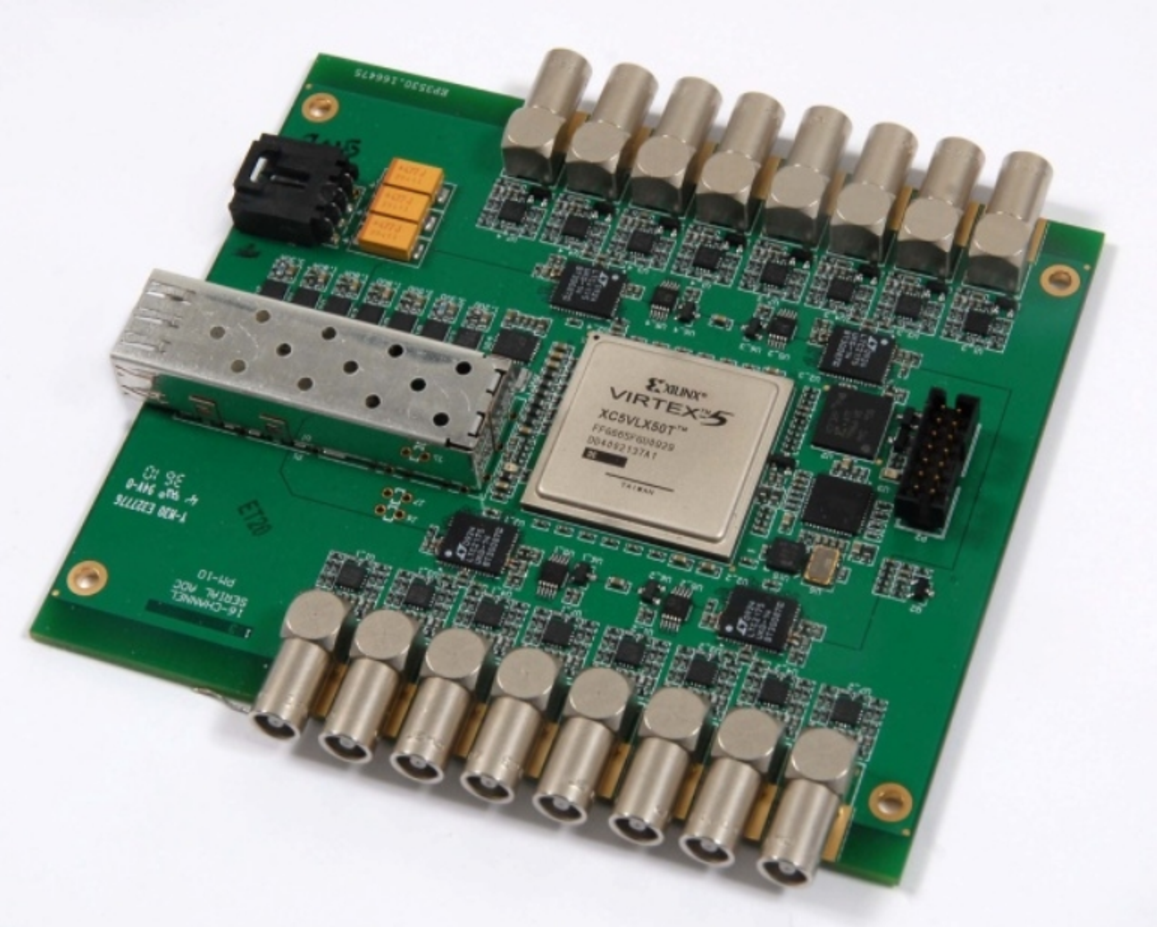
\includegraphics[width=\linewidth]
{fig/virtex5.pdf}
\vspace{1em}
\caption{}
\end{subfigure}
\begin{subfigure}[b]{0.3\linewidth}
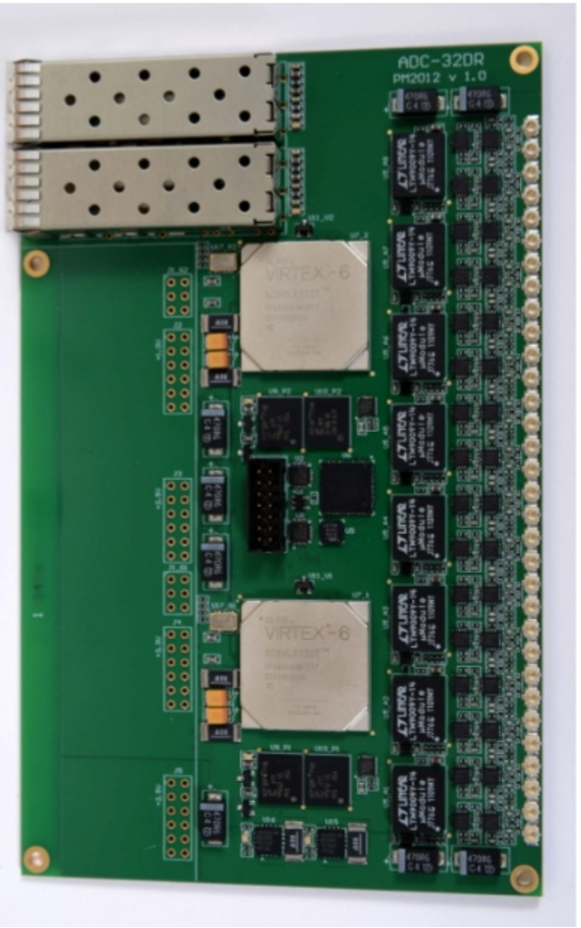
\includegraphics[width=\linewidth]
{fig/virtex6.pdf}
\caption{}
\end{subfigure}
\begin{subfigure}[b]{0.33\linewidth}
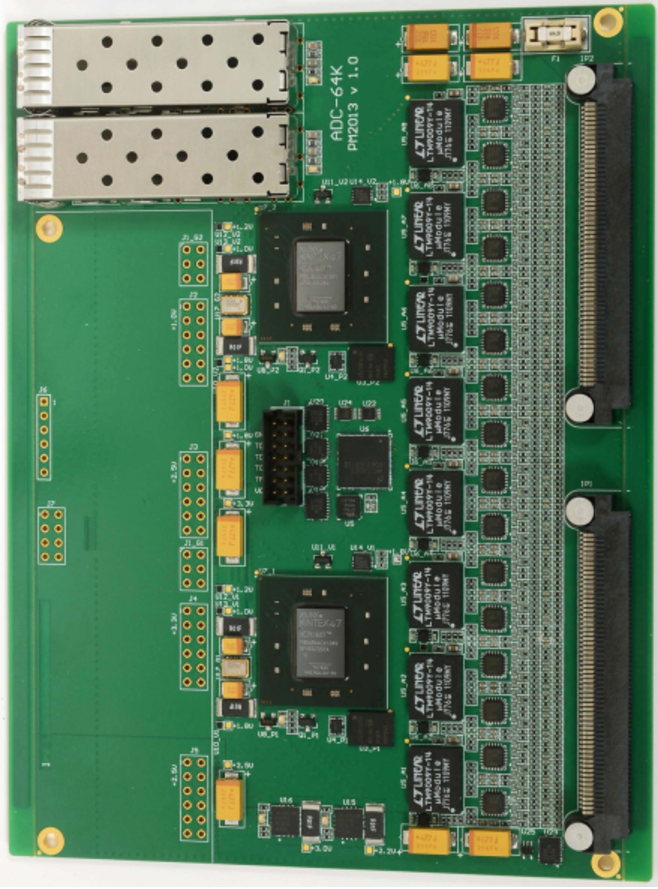
\includegraphics[width=\linewidth]
{fig/kintex7.pdf}
\caption{}
\end{subfigure}
\caption{ADC portfolio. \\
(a) 16-channel, 125 MSPS, Virtex-5 based\\
(b) 64-channel, 80 MSPS, Virtex-6 based\\
(c) 64-channel, 80 MSPS, Kintex-7 based}
\label{fig:sadc:board}
\end{figure}
The limited space provided in the detector for the ADC system requires high channel density and liquid cooling of the devices. 
In order to define the optimal design for the task, a number of different 14-bit sampling ADC modules were constructed, see \Reffig{fig:sadc:board}. The ADC portfolio includes a 16-channel, 125\,MS/s table-top module, a 64-channel, 80\,MS/s dual-range high-end module and a 64-channel, 80\,MS/s economy module \cite{kavatsyuk}. 
\section{Module construction}
The 64-channel ADCs are equipped with symmetrizing shapers/amplifiers allowing for user defined CR-(RC)$^3$ filter configurations. In configurations with by-passed CR-(RC)$^3$ filter, the input analog stage features over \SI{100}{\mega\hertz} bandwidth. Obtaining a 14-bit dynamic range required by the PANDA experiment was found to be feasible through using a dual-range ADC structure. By fitting SMD jumpers, a 32-channel dual range configuration can be obtained.
Amplified signals are processed by a set of 8-channel 14-bit, 80\,MS/s analog-to-digital converter circuits, see \Reffig{fig:sadc:structure} 

\begin{figure}[htb]
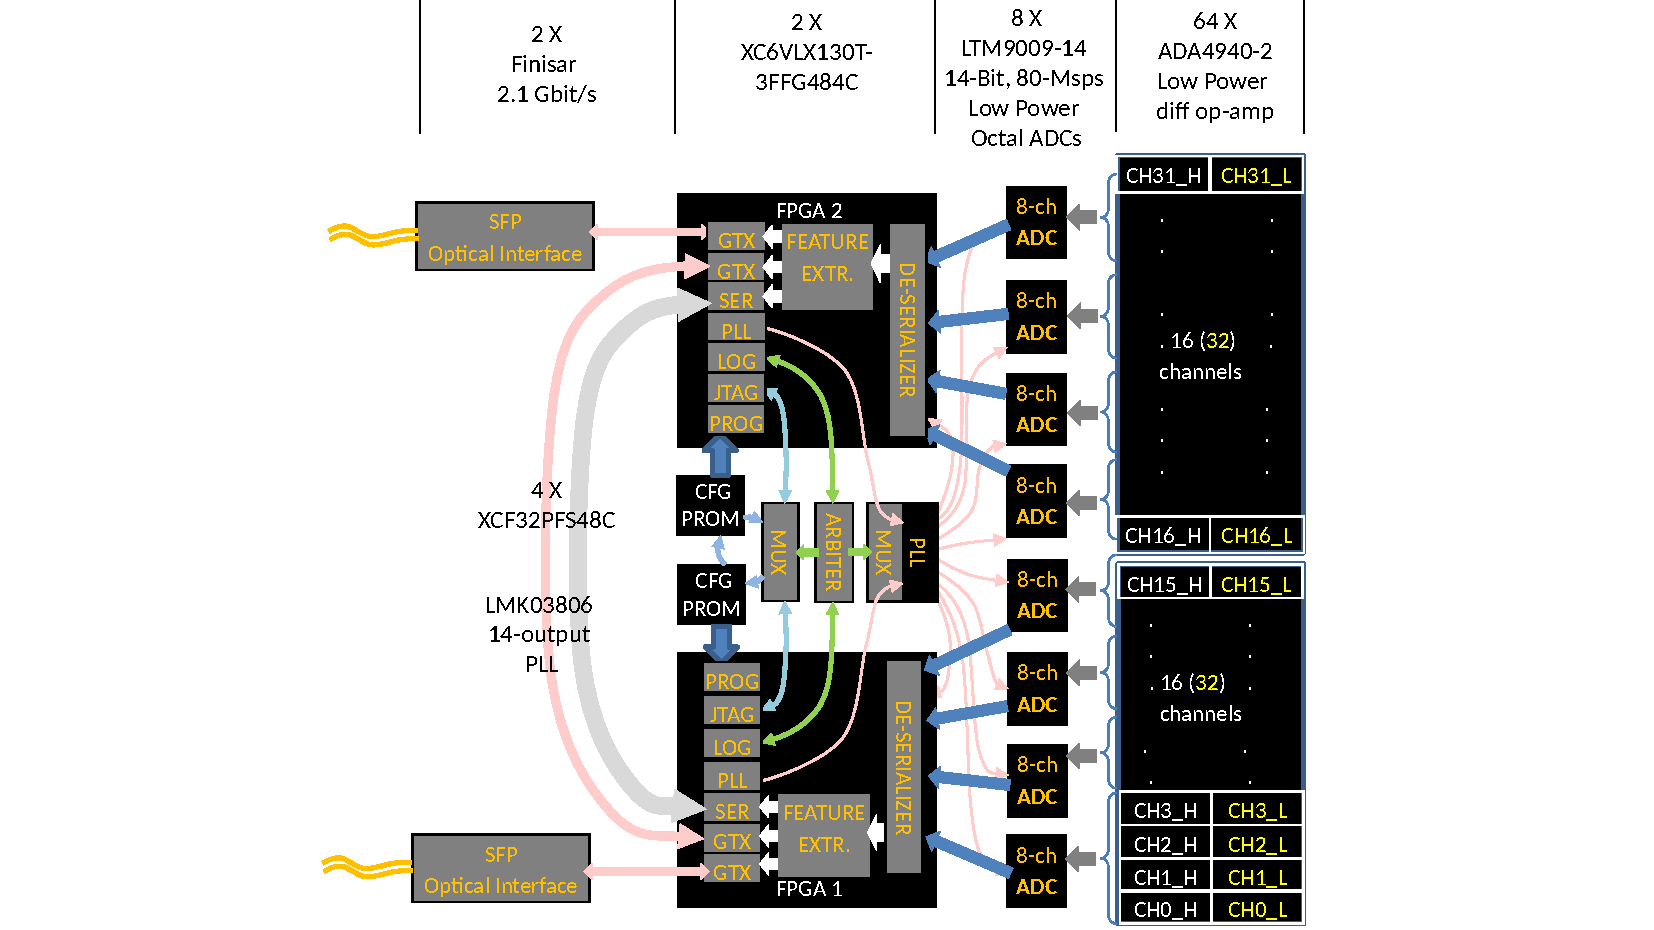
\includegraphics[width=\linewidth, trim={120 0 120 0}, clip]{fig/hardware.pdf}
\caption{Hardware structure of the \panda  Sampling Analogue-to-Digital Converter board (SADC).}
\label{fig:sadc:structure}
\end{figure}

Digitized samples of 64 analog signals are sent to 2 FPGAs using 128 LVDS links running at 560\,Mbit/s each. 
The FPGA firmware performs signal filtration, and extracts important signal parameters, such as time of arrival, amplitude and integral. 
The data assembled in output registers are pushed to the optical links via multi-gigabit transceivers (GTX) running at 2\,Gbit/s. Depending on data rate and firmware configuration, it is possible to use either both optical links, which are independently controlled by 2 FPGAs or use only one optical link and inter-FPGA serial or parallel data connections.
The ADC module is compliant with the SODA System, for which the reference clock is distributed via a DAQ, using the down-link part of the ADCs optical transceiver. It allows for obtaining defined latencies with a reference time accuracy of \SI{50}{\pico\second} \cite{konorov}. The received reference clock signal is routed out from the FPGAs and processed by a 14-output PLL/jitter cleaner circuit, providing a set of stable clocks for all digitizers as well as for all GTX inside FPGAs. 
A dual FPGA structure and a hardwired arbitration circuit provide routing of the JTAG configuration signals to the FPGAs and control of the reference clock source. This allows for resolving potentially catastrophic situations, when a content of a configuration memory is damaged by radiation in such a way that the loaded configuration affects the communication chain, thus locking the possibility for a remote repair of the faulty content.
The dimension of 64-channel modules amounts to \SI{100 x 150}{\squared\milli\metre}, including the area designated for DC/DC converters. Despite a high channel density, no measurable crosstalk has been observed. The proximity of specially designed DC/DC converters also doesn’t give any measurable rise to the signal noise. The power consumption amounts to \SI{22}{\watt} for the  Kintex-7 version and \SI{27}{\watt} for the Virtex-6 version. This requires efficient cooling, which in the PANDA will be accomplished by liquid-cooled aluminum encapsulations.
\section{ADC test and measurement setup}
The test setup was based on a firmware developed for the Crystal Barrel experiment at the Bonn University. The firmware allows self-triggering with variable threshold, as well as external trigger and network-based trigger. Several algorithms for pulse integral determination, peak-sensing and digital constant fraction discrimination allow to characterize the waveform such that it's properties can be determined efficiently with regards to memory and bandwidth. Additionally, the transmission of full samples with a length of \SI{12.8}{\micro\second} is possible for any channel. With the versatile AXI interface, the data-streams are handed over to a 1GB/s UDP/IP core, based on an open source code (opencores.org, BSD). The usage of Ethernet with UDP/IP has allowed for a great simplification of lab setups, introducing the possibility to directly connect the SADC to a computer. 
\begin{figure}[htb]
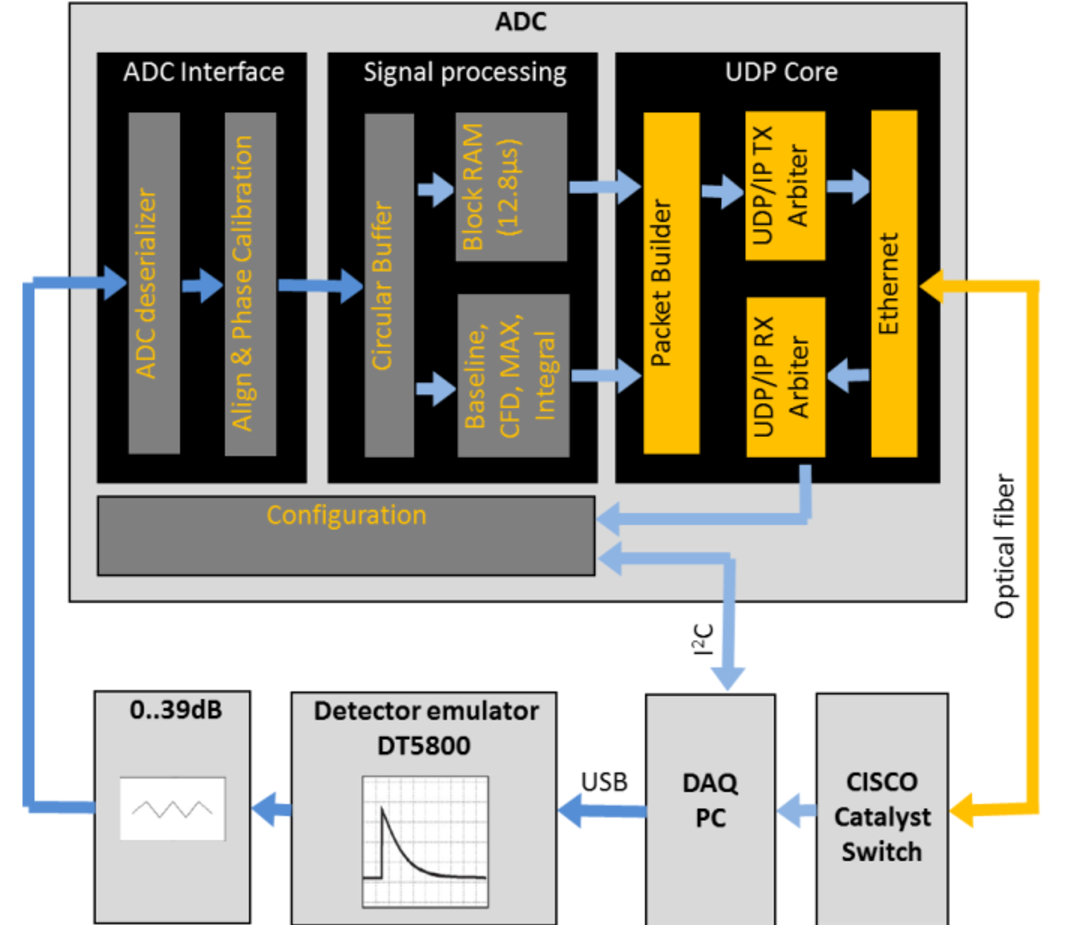
\includegraphics[width=\linewidth]{fig/ADCsetup.pdf}
\caption{ADC and detector performance test setup.}
\label{fig:sadc:setup}
\end{figure}
Data taking as well as configuration can be done within one simple framework, see \Reffig{fig:sadc:setup}. The setup was used for evaluation of the detector sensitivity and noise, as well as for performance analysis of the ADC module.
\section{Performance of the ADC analog stage}
Given the light yield of the PbWO4 crystals, the quantum efficiency, the gain of the photo-sensors, as well as the pre-amplifier gain, the signals amplitude at the ADC inputs corresponding to energy depositions of \SI{1}{\mega\electronvolt} to \SI{12}{\giga\electronvolt} will range from \SI{160}{\micro\volt} to \SI{2.2}{\volt} respectively. To achieve a high resolution of the ADC, every detector signal is processed by a high-gain and a low-gain channel, see \Reftbl{tab:ADCanpref}.
\begin{table}[htb]
\caption{\label{tab:ADCanpref}ADC analog performance.}
\begin{center}
	\begin{tabular}{p{2cm}cc}
	Parameter&Low Gain&High Gain \\ \hline
	Gain&0.5&7.2 \\ \hline
	\multirow{2}{2cm}{Input amplitude} & $<$ \SI{ \pm2.2}{\volt} & $<$ \SI{ \pm0.14}{\volt} \\
	& (0 -- \SI{12}{\giga\electronvolt}) & (0 -- \SI{1}{\giga\electronvolt})\\ \hline
	\multirow{2}{2cm}{Noise}&\SI{1.3}{\milli\volt}&\SI{0.08}{\milli\volt} \\
	&(\SI{8}{\mega\electronvolt}) &(\SI{0.5}{\mega\electronvolt}) \\ \hline
	Bandwidth&$>$ \SI{100}{\mega\hertz}&$>$ \SI{20}{\mega\hertz}\\ \hline
	Linearity&\multicolumn{2}{c}{ 0.6~\%}\\ \hline
	Amplitude Resolution&\multicolumn{2}{c}{ $<$ 0.1~\%} \\ \hline
	Charge Resolution&\multicolumn{2}{c}{ $<$ 0.1~\%} \\ \hline
	\end{tabular}
\end{center}
\end{table}
The noise, linearity, amplitude and charge resolution figures were measured at Ruhr-University Bochum with the help of a detector emulator device (CAEN DT5800), which was configured to deliver pulses comparable to the preamplifier signals in the experiment. The ADC was set to a self-triggered mode of operation. The baseline was calculated using the moving average of 200 samples preceding the signal.
The RMS noise of the ADC in high-gain channels amounts to \SI{0.08}{\milli\volt} (\SI{0.5}{\mega\electronvolt}), while the baseline amplitude distribution has a white noise character and does not show signs of the interference from the digital part of the device, see \Reffig{fig:sadc:noise}.
\begin{figure}[htb]
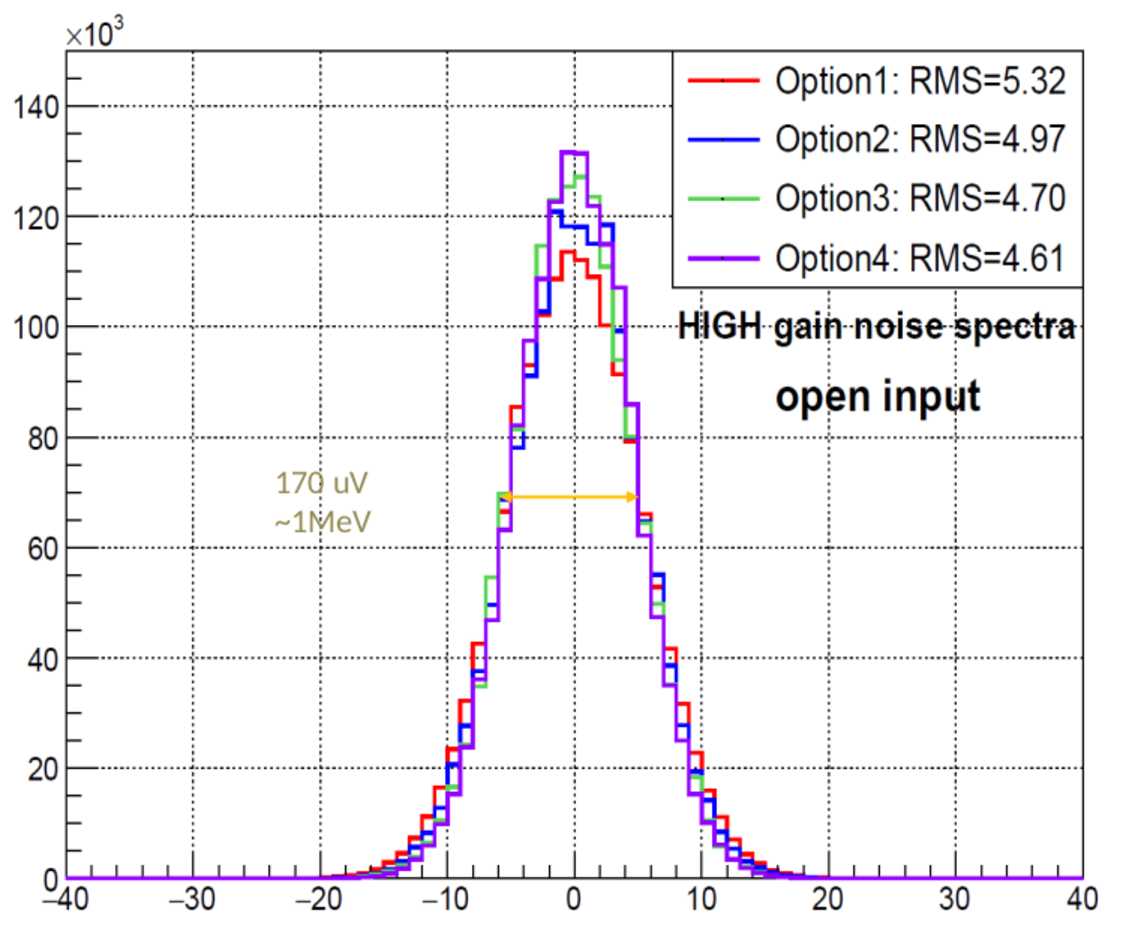
\includegraphics[width=\linewidth]{fig/ADCnoise.pdf}
\caption{The ADC noise with optional high-pass filters. With 58 bins per 1 MeV in the high-gain channel, the RMS noise amounts to 80µV.}
\label{fig:sadc:noise}
\end{figure}
\section{Performance of the ADC sampling}
\begin{itemize}
\item Example of a digitized waveform with a light pulser \Reffig{fig:sadc:example}.
\item Example of a digitized waveform with cosmics.
\item Example of a digitized waveform with a neutron/proton/gamma beam.
\item Time/Energy resolution for each example.
\item Different waveforms for several energy values  and Low/High gain could be shown.
\end{itemize}
\begin{figure*} [htb]
\begin{subfigure}[b]{0.5\linewidth}
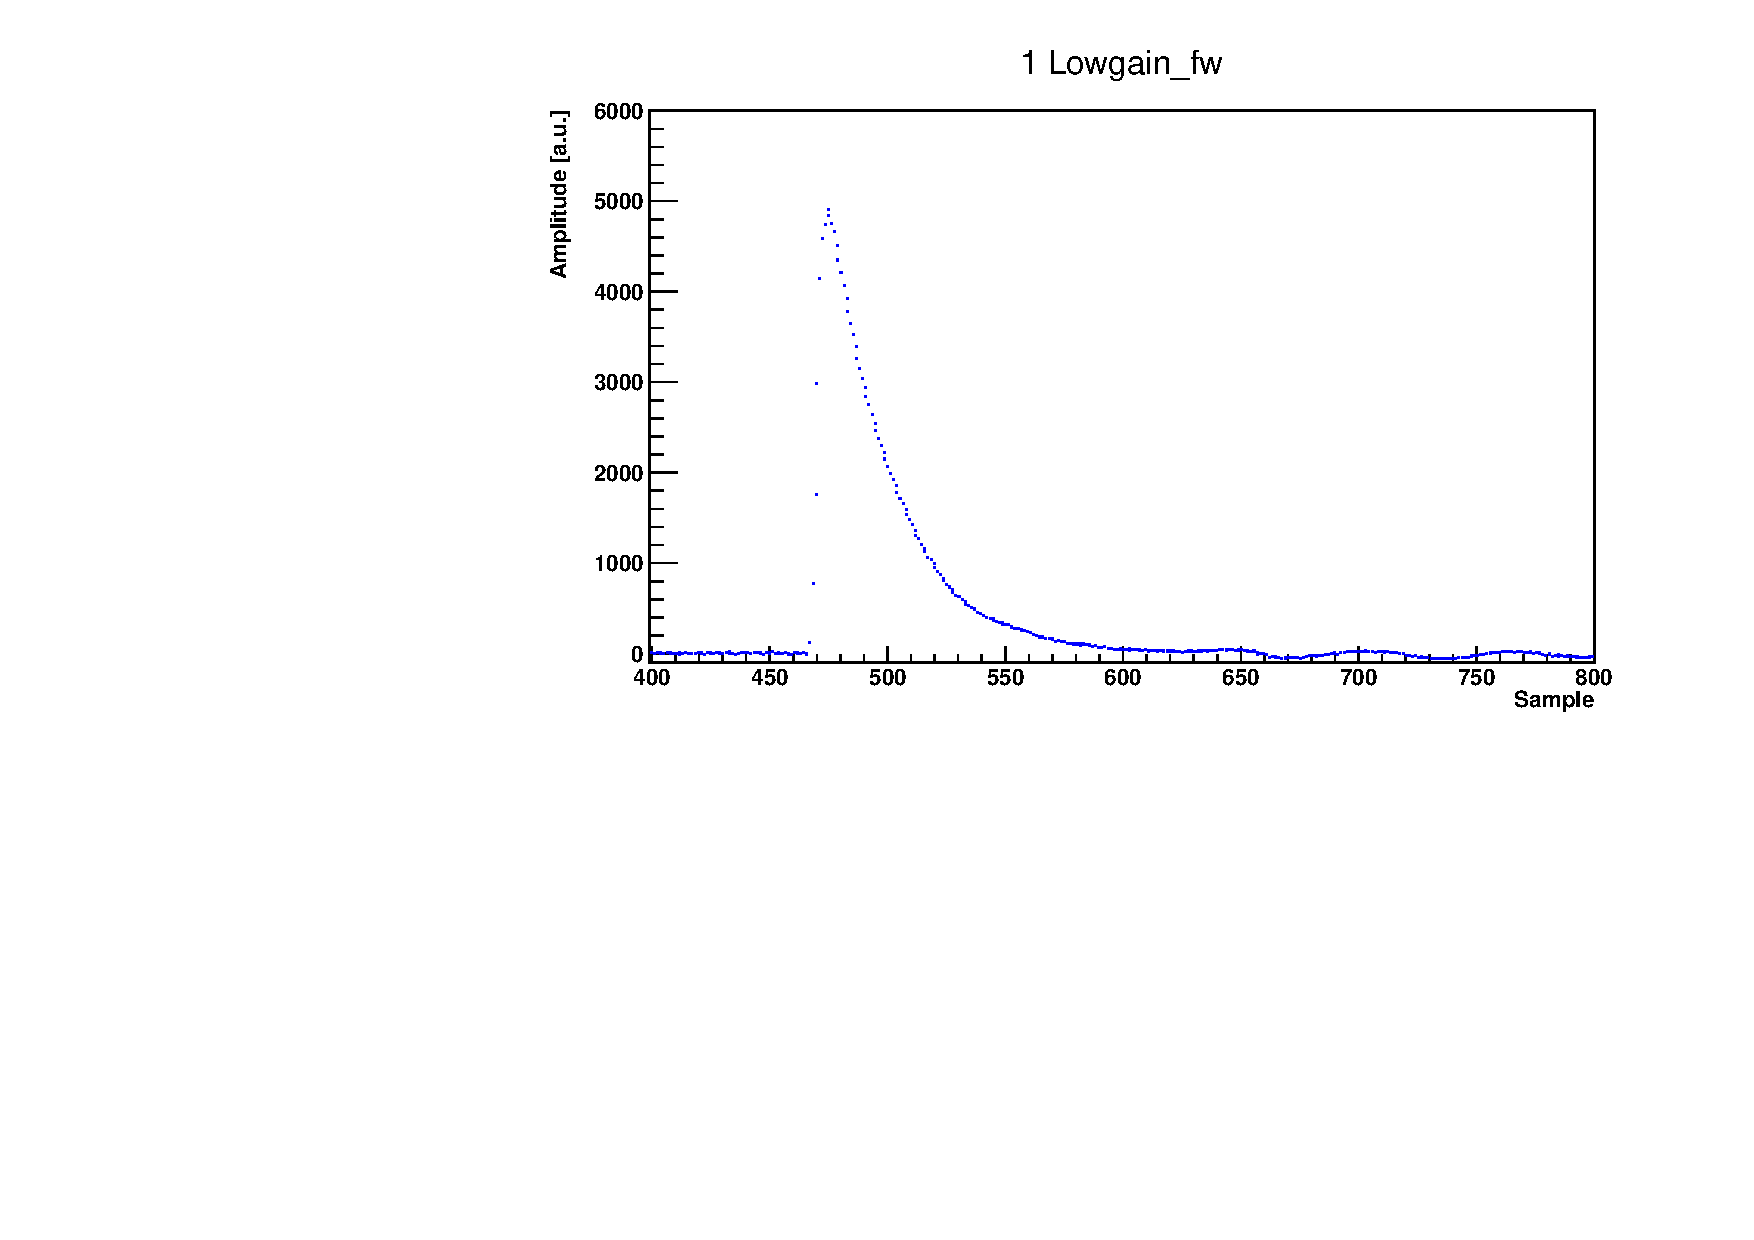
\includegraphics[width=\linewidth]{fig/Lowgain814.pdf}
\caption{Lightpulser, Lowgain 2.2V (12 GeV).}
\label{fig:sadc:2.2V_Low}
\end{subfigure}
\begin{subfigure}[b]{0.5\linewidth}
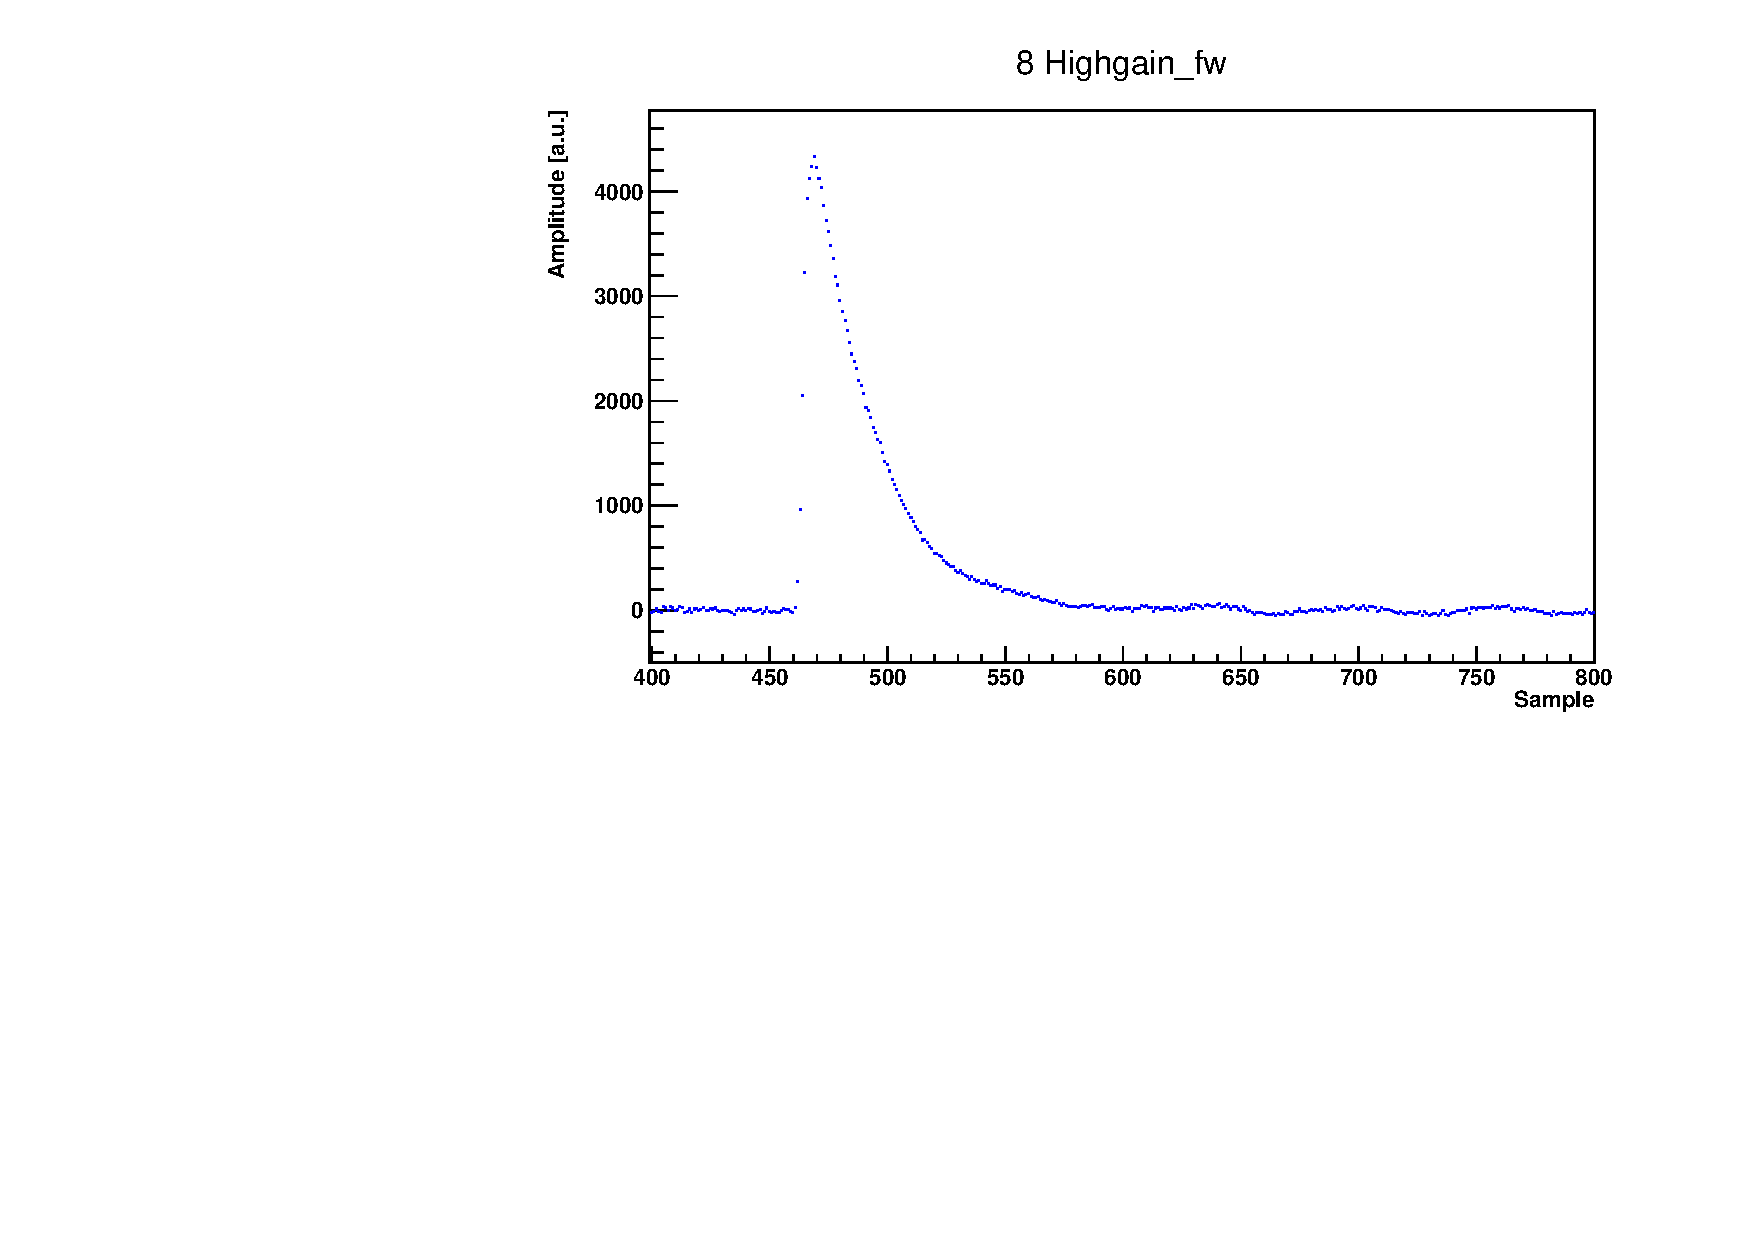
\includegraphics[width=\linewidth]{fig/Highgain815.pdf}
\caption{Lightpulser,Highgain 48mV (262 MeV).}
\label{fig:sadc:48mV_High}
\end{subfigure}
\\
\begin{subfigure}[b]{0.5\linewidth}
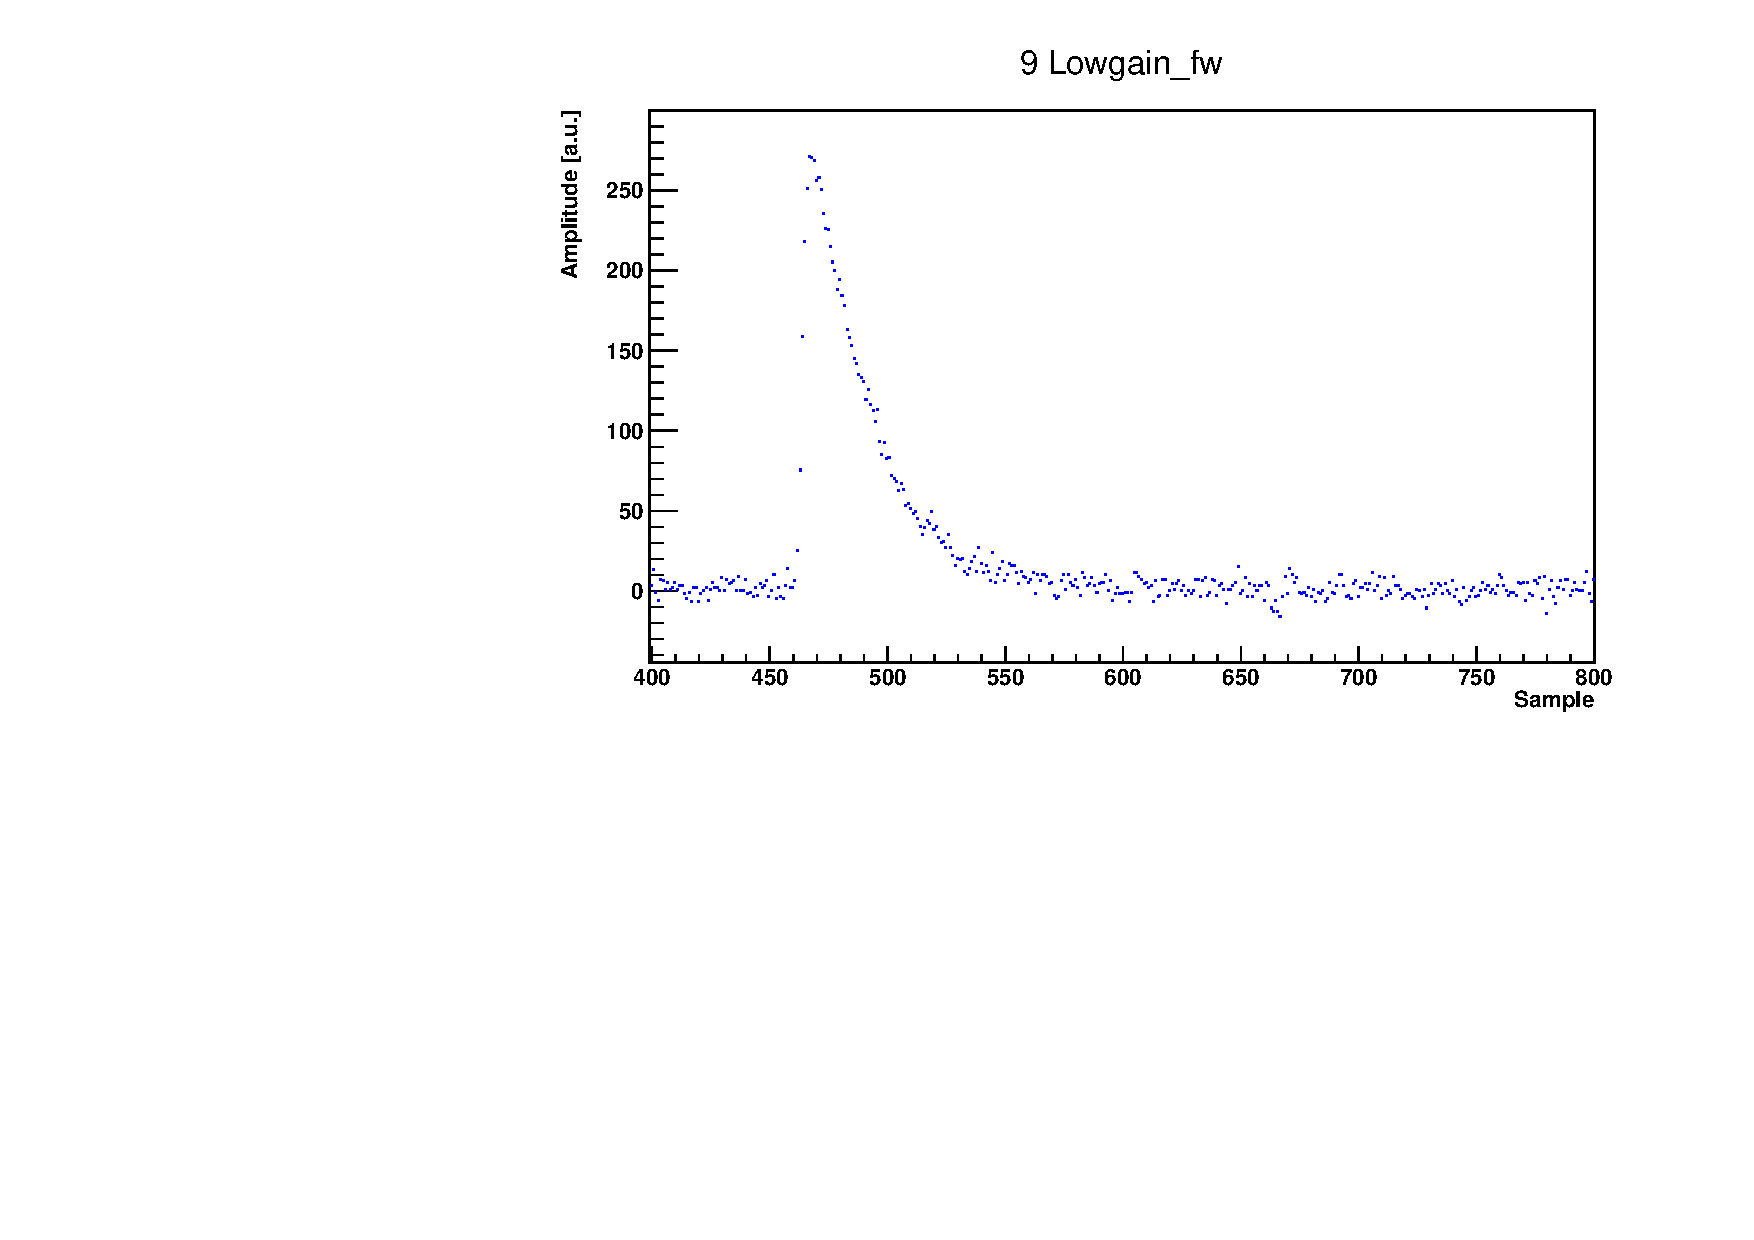
\includegraphics[width=\linewidth]{fig/Lowgain815.pdf}
\caption{Lightpulser, Lowgain 48mV (262 MeV).}
\label{fig:sadc:48mV_Low}
\end{subfigure}
\caption{Waveforms example.}
\label{fig:sadc:example}
\end{figure*}
\section{Analog and digital signal filters}
This part of the design is under evaluation with the goal to detect energy spills as low as \SI{3}{\mega\electronvolt} as well as resolve and parametrize signal pileups occurring with down to \SI{200}{\nano\second} time separation with the best achievable time and energy resolution.
Detecting the weakest signals requires signal filtration, while the optimal filter parameters depend on the expected particle rate in the detector. In case of low rates, adequately longer signal shaping constants result in better signal to noise ratio, hence in better energy resolution and wider dynamic range, see \Reffig{fig:sadc:filter}. 
\begin{figure}[htb]
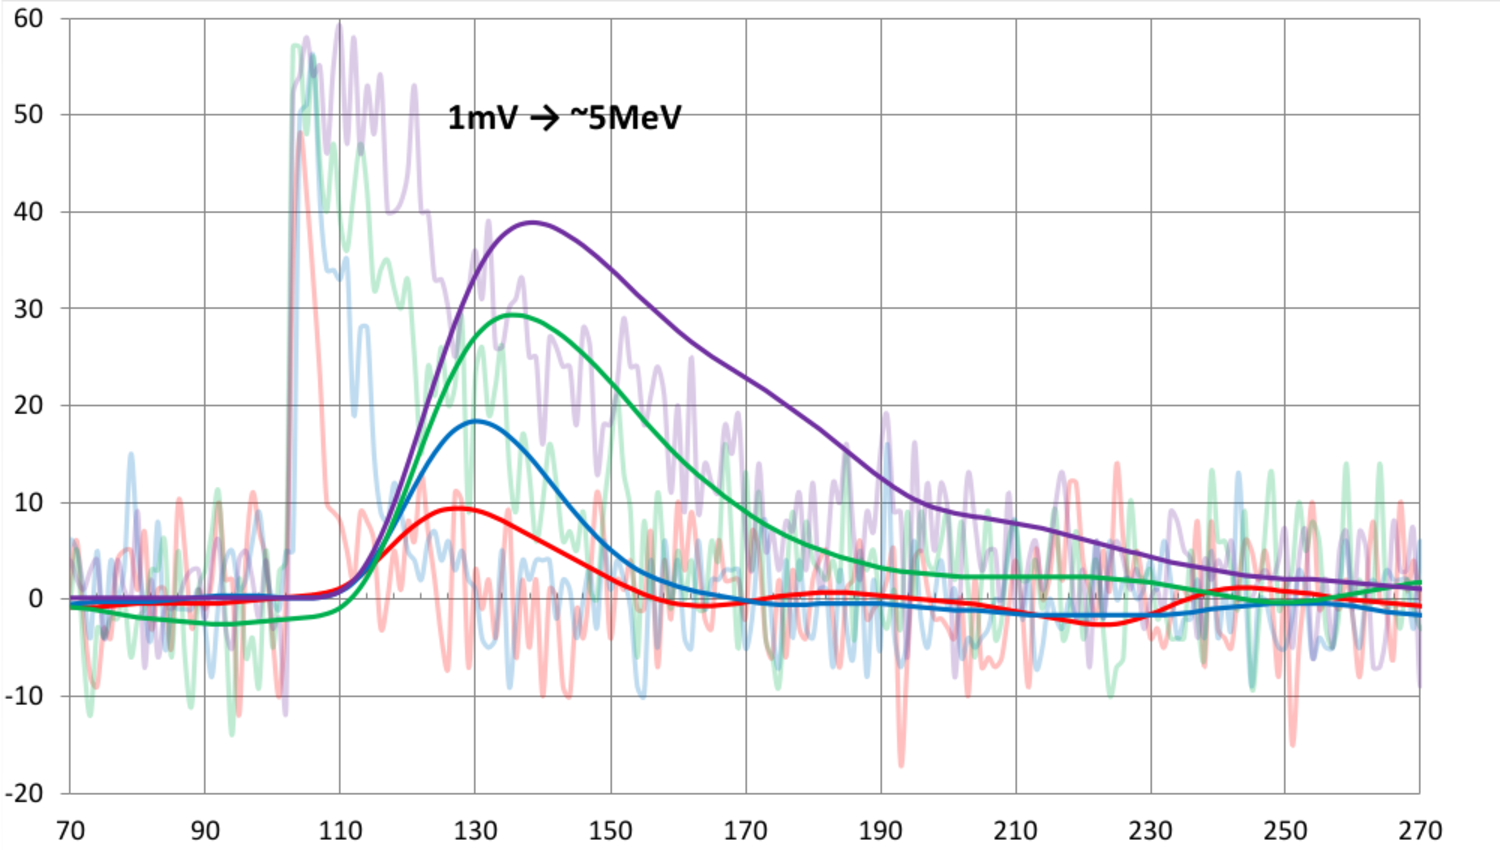
\includegraphics[width=\linewidth, trim={3 3 0 0}, clip]{fig/ADCfilter.pdf}
\caption{A \SI{1}{\milli\volt} analog signal (corresponding to \SI{5}{\mega\electronvolt} energy deposition). }
\label{fig:sadc:filter}
\end{figure}
Signal filtration methods for higher rates as well as multiple pulse detection and parametrization using Moving Window Deconvolution (MWD), Moving Averaging (MA) and Constant Fraction Timing (CFT) were developed and tested at KVI-CART, Groningen, The Netherlands \cite{Tambave_2012}. 
The ADCs were successfully tested with a readout system running the SODANET protocol. 
\section{Feature Extraction Firmware on the SADC module}
The feature extraction algorithm was designed for implementation on the developed SADC module, which is required to process signals at high interaction rates. The signal filters mentioned in a previous section  are used for efficient signal processing during the feature extraction procedure. 

Implementation of the feature extraction algorithm on the FPGA is done in VHDL. The signal-processing logic is shown as a block diagram in \Reffig{fig:fea_fwendcap}. 
\begin{figure}[h]
    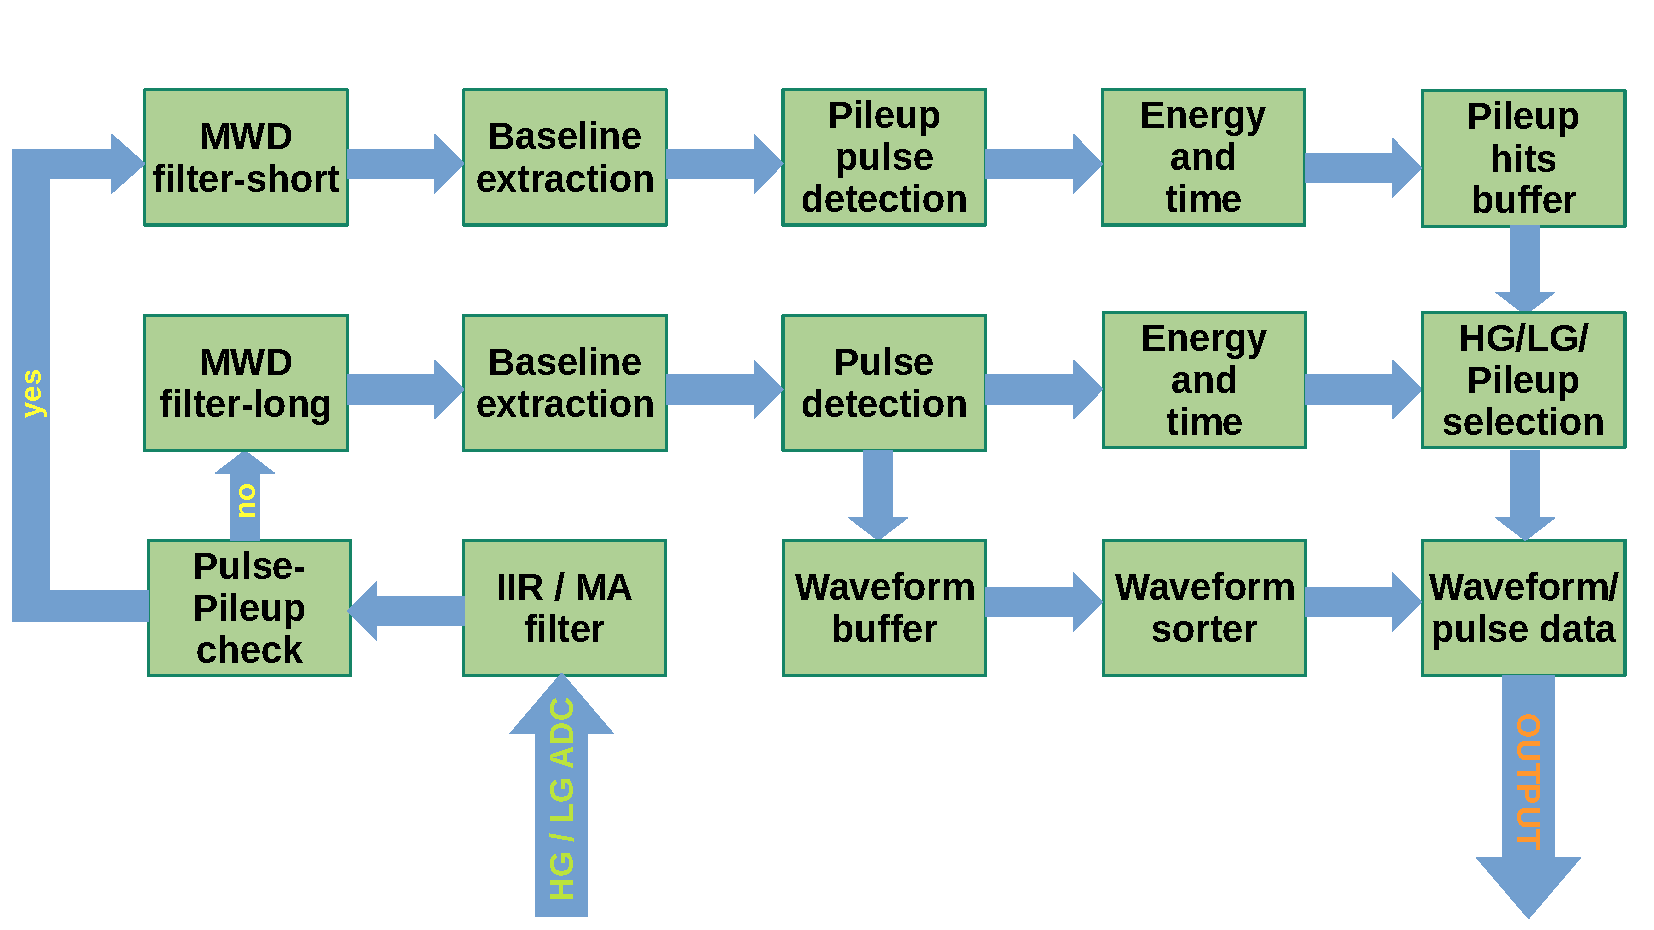
\includegraphics[width=0.49\textwidth ,trim={0 0 0 0}, clip]{fig/Scheme_FE.pdf}
    \caption[Scheme of the Feature Extraction Algorithm implemented on ADC]{
    The block diagram of the feature extraction algorithm implemented on the FPGA of the sampling ADC.}
    \label{fig:fea_fwendcap}
\end{figure}
The digitized waveforms from high and low gain ADC channels, i.\,e.\@ pulses, are simultaneously processed by the feature extraction algorithm. \\At the beginning, the high (low) gain signal is sent to the Infinite Impulse Response (IIR) filter, which is similar to the MA filter. They are used for signal smoothing and noise reduction leading to precise pulse detection at lower thresholds. There is possible to select by the slow control system which of them will be used for the feature extraction.  branch with the MWD II functional block is used to reduce the pulse length even more in comparison to MWD I. Thus, these two blocks reduce the processing time of the waveform, which decreases the probability of signal pile-up at high rates. 
The next component, Pulse-Pileup check, performs several functions. Firstly, it discards the digitized waveforms which do not have enough samples
The following Feature-Extraction module (FE) has the same structure for both. Discrete-in-time samples of the digitized waveform are passed through the baseline functional block (Baseline), which restores the correct baseline for precise energy determination. The output of the baseline block is connected to three readout functional blocks, namely to Trigger (Tr), CFT and MA filter.
The MWD functional block provides the time-stamp information. The MA functional block is used for smoothing and noise reduction leading to precise pulse detection at lower thresholds. If the sample-value is higher than the set threshold in the Tr block, this block sends a command to process the information given by the CFT and MA blocks after each sample from now for the Time-Energy determination in the Time and Energy (E) functional blocks. The Tr block performs not only the detection of the pulse but also its interruption. When the sample-value becomes lower than 1/4 of the threshold value, this block sends a command to stop the time-energy determination. As a result, the time and energy values, extracted from the pulse, are propagated to the last functional block: Pileup Identification and Recovery (I/A). This block is used to estimate the integral/amplitude ratio. If this ratio is bigger than a value set by the user, the output is taken from the parallel branch with a shorter 
waveform after the MWD block. Received time-energy data are sent to the Data Concentrator (DC).
\section{Test of the ADC module in a test beam environment}
The ADC was used in a detector setup for testing response of EMC Forward End-Cap PbWO4 crystals to photons with energies from \SIrange{10}{62}{\mega\electronvolt}. In the experiment performed at Max Lab III in Lund, 2014, a 3 x 3 matrix of crystals was equipped with Hamamatsu R11375 Vacuum Photo-Tetrodes (VPTT) and SP883d signal preamplifiers from the University of Basel \cite{Keshelashvili_2015}. The signals were processed by the Virtex-6 ADC version equipped with 300ns input shaping filter. The waveform data were transferred to a PC via a VME-based Data Concentrator module (ATLB) \cite{Marciniewski}.
After off-line energy reconstruction and applying \SI{1.5}{\mega\electronvolt} thresholds, the relative energy resolution obtained for photon energies of \SIlist{11; 26; 38; 62}{\mega\electronvolt} was found to be fulfilling the Technical Design Report requirements of the PANDA EMC with a safety margin, \Reffig{fig:sadc:resolution}.

\begin{figure}[htb]
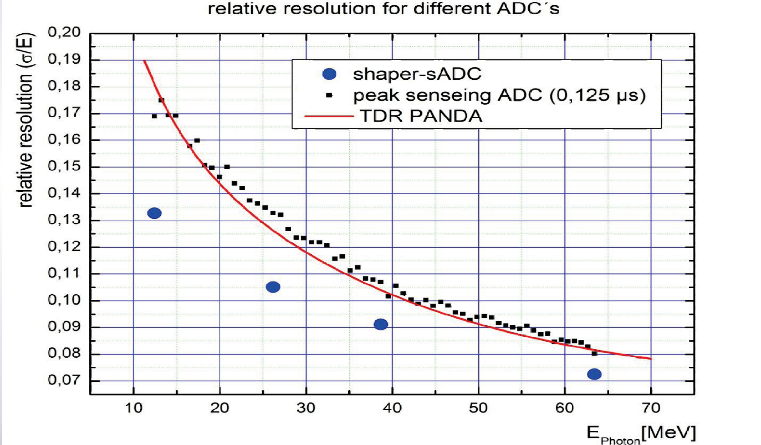
\includegraphics[width=0.49\textwidth ,trim={1 0 0 0}, clip]{fig/Figure3.png}
\caption{\label{fig:sadc:resolution}Calorimeter energy resolution for low energy photons.}
\end{figure}
\section{Neutron irradiation of the ADC}
In order to test the endurance of the ADC in a radiation environment, the Kintex-7 version of the device was irradiated with a neutron beam at The Svedberg Laboratory (TSL), Uppsala University in June 2016. The purpose of this experiment was to find the cross section of the device for the SEU-induced bit errors and estimate the Mean Time Between Failures (MTBF) of the device when placed inside of the operating PANDA detector.
The neutron beam was produced by directing a \SI{180}{\mega\electronvolt} proton beam into a full-stop tungsten target.
The ADC was first placed at the Standard User Position (SUP), perpendicular to the beam which had a diameter of \SI{130}{\milli\metre}. The neutron flux $\Phi_n$  ($>$\SI{10}{\mega\electronvolt}) at this position amounted to $5\times10^5$ -- $10^6 s^{-1}cm^{-2}$  with the energy spectrum as shown in \Reffig{fig:sadc:irradiation}.

\begin{figure}[htb]
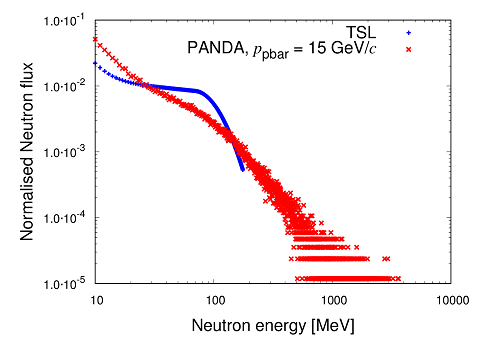
\includegraphics[width=0.49\textwidth, trim={0 2 3 0}, clip]{fig/Figure4.png}
\caption{\label{fig:sadc:irradiation}Neutron energy spectrum at the TSL (blue) and the anticipated in the \panda (red).}
\end{figure}
During the experiment, the Xilinx Soft Error Mitigation (SEM) Controller was placed in the FPGA \cite{xilinx}. The SEM Controller has the ability to detect and correct different types of SEUs and its activity was monitored via a serial link.
In this experiment, the SEM was automatically correcting Single-Bit Upsets (SBU) as well as Multiple-Bit Upsets MBU, spread over multiple frames in the FPGA memory (inter-frame). MBU located in the same frame (intra-frame) are not automatically correctable by SEM and require reconfiguration of the affected FPGA, which causes an FPGA dead time of the order of \SI{200}{\milli\second}.
\begin{figure}[htb]
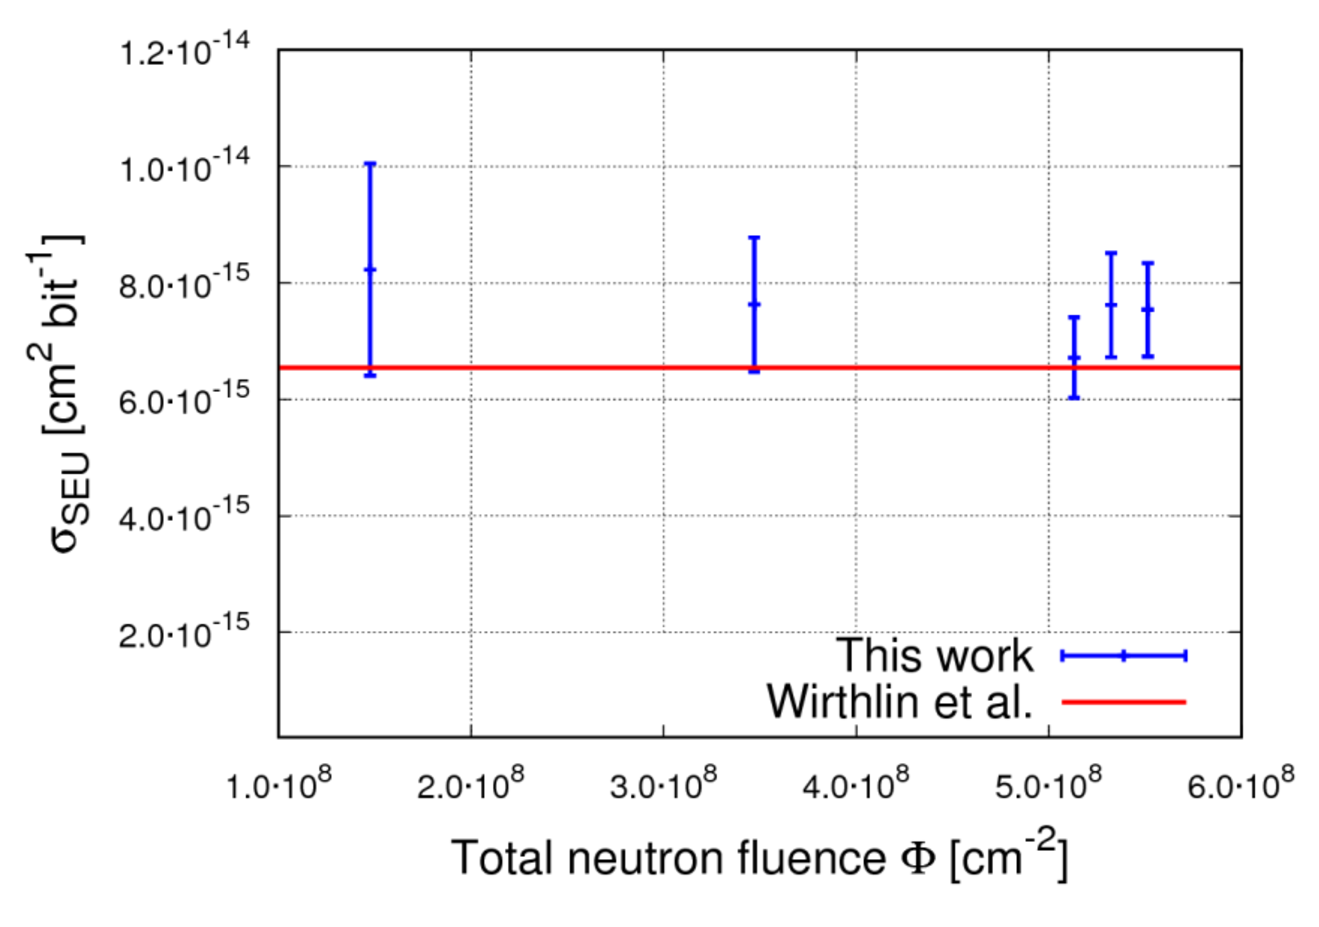
\includegraphics[width=0.49\textwidth, trim={0 0 0 0}, clip]{fig/ADCcssneutron.pdf}
\caption{\label{fig:sadc:cssneutron} SEU cross sections of the ADC (FPGA) for neutrons.}
\end{figure}
The occurrence of the SBU amounted to 69~\%, inter-frame MBU -- 26~\% and intra-frame MBU -- 5~\%.
After dividing the registered SEU number by beam time and normalizing the result to the neutron flux we have obtained:
\begin{equation} \label{eq1}
\begin{split}
\sigma_{SEU}&=\frac{N_{SEU}}{T_{MEAS}\cdot \Phi_n\cdot N_{BITS}}=\\
&=7.42\cdot 10^{-15} cm^2\cdot bit ^{-1}
\end{split}
\end{equation}
per FPGA, which is in agreement with the results achieved by a group of M. J. Wirthlin \cite{Wirthlin_2014}, see \Reffig{fig:sadc:cssneutron}. 
In order to find the MTBF in PANDA, a simulation of the neutron flux in the EMC was made using a PandaRoot simulation package \cite{Messchendorp:2010zz}. Given the beam momentum P$_{pbar}$ = \SI{15}{\giga\electronvolt\per\clight}
 and a luminosity of $L$= $2\cdot10^{32}cm^{-2}s^{-1}$, the scaled neutron flux at the position of the digitizers in PANDA amounts to 
$\Phi_n$ = 150 $s^{-1}cm^{-2}$
\section{Proton irradiation of the ADC}
In November 2016 the ADC board was irradiated with a proton beam delivered by the AGOR cyclotron at KVI, Groningen. The beam was collimated with a \SI{120}{\milli\meter} collimator, illuminating a top half of the digitizer board, including one of the FPGAs and SFP optical transceivers. 
Irradiations of an older prototype of the ADC, based on the Virtex-6 FPGA, have been performed at KVI-CART in the past \cite{kava2}. The new measurements were done at proton energies of \SIlist{80; 100; 184}{\mega\electronvolt}, allowing for studies of the energy-dependence of the SEU cross section. 

\begin{figure}[htb]
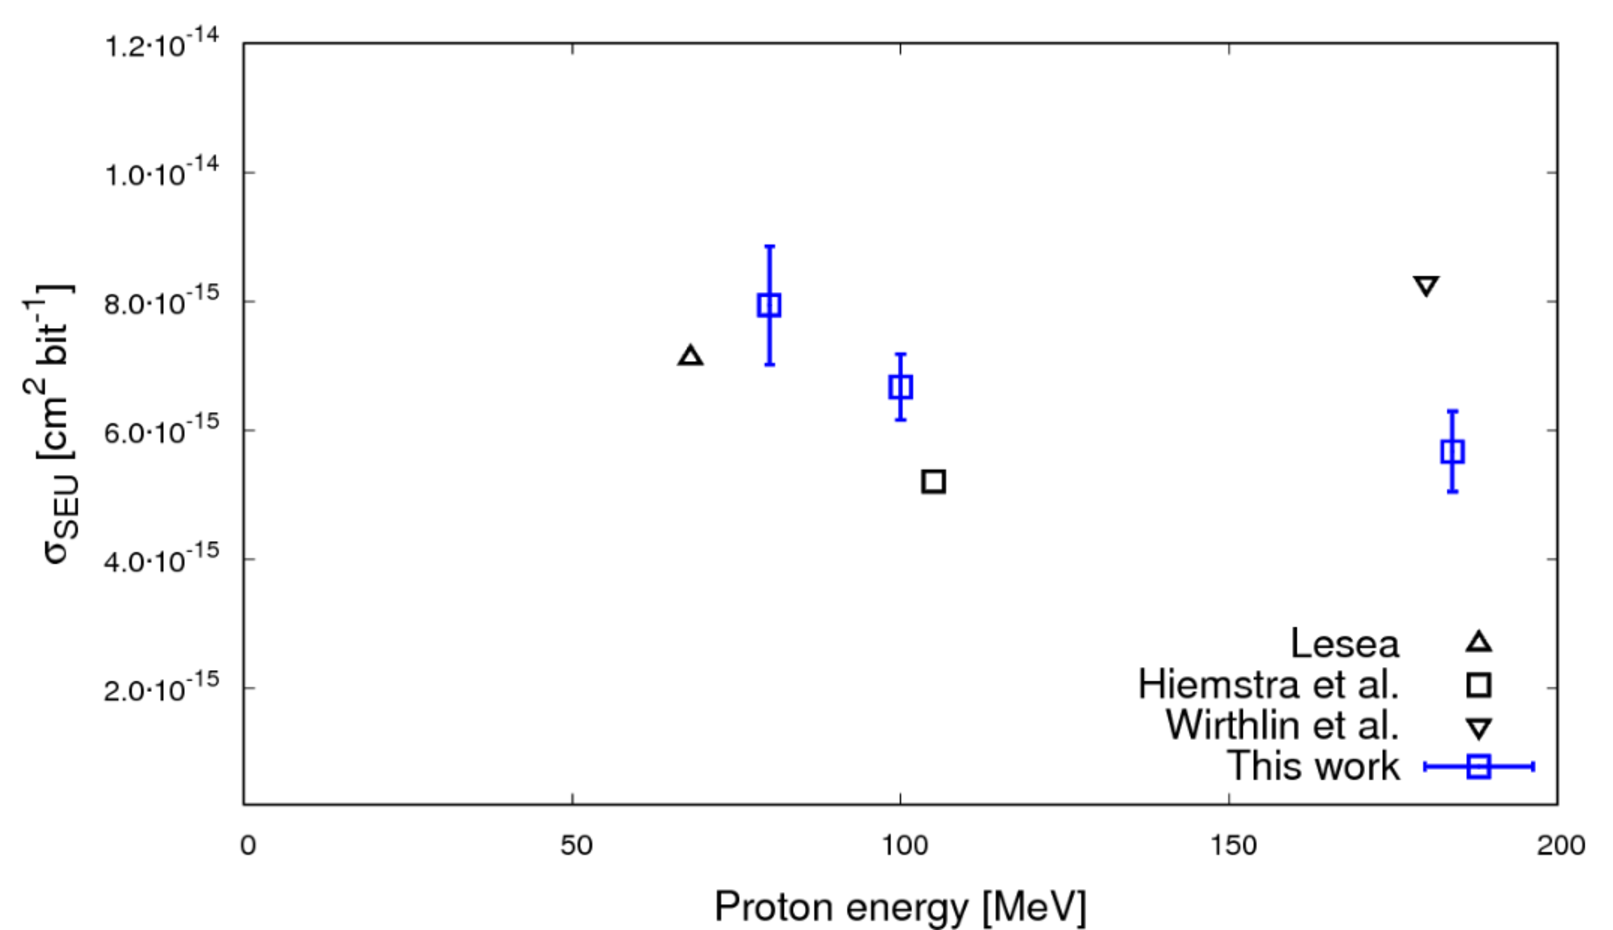
\includegraphics[width=\linewidth, trim={0 0 0 0}, clip]{fig/ADCcssproton.pdf}
\caption{\label{fig:sadc:cssproton}SEU cross sections of the ADC (FPGA) for protons.}
\end{figure}
By using the same analysis procedure as for the neutron-irradiation data, the obtained cross-sections for a Xilinx XC7K-160T FPGA are summarized in \Reftbl{tab:Crss}. These results agree with previously reported measurements by Hiemstra et al., Leslea et al. and Wirtlin et al., see \Reffig{fig:sadc:cssproton} \cite{tale},\cite{kintex}. 
\begin{table}[htb]
\caption{\label{tab:Crss}Cross sections for proton-induced SEUs at different beam energies for XC7K-160T.}
\begin{center}
	\begin{tabular}{c|c}
	$E_{pbeam}$ [MeV]&$\sigma_{SEU}$ [$cm^2\cdot bit ^{-1}$] \\ \hline
	80 & $7.94\cdot10^{-15}$ \\ \hline
	100 & $6.67\cdot10^{-15}$ \\ \hline
	184 & $5.67\cdot10^{-15}$ \\ \hline
	\end{tabular}
\end{center}
\end{table}
The total number of impact protons on the device during the proton irradiation session amounted to $1.12\cdot10^{10}cm^{-2}$.
The flux of high-energy charged particles in the PANDA experiment at the location of the ADC modules was also simulated with the PandaRoot framework \cite{kava2} and amounts to 
$\Phi_p$ = 60 $s^{-1}cm^{-2}$.
The device was thus exposed to a dose equivalent of 6.5 years of detector operation at high luminosity. After the test, the device is still fully functional and no measurable degradation of performance was observed. 
\section{ADC recovery after irradiation}
Recovery of the SADC board from the radiation damage requires time. 
\begin{figure}[htb]
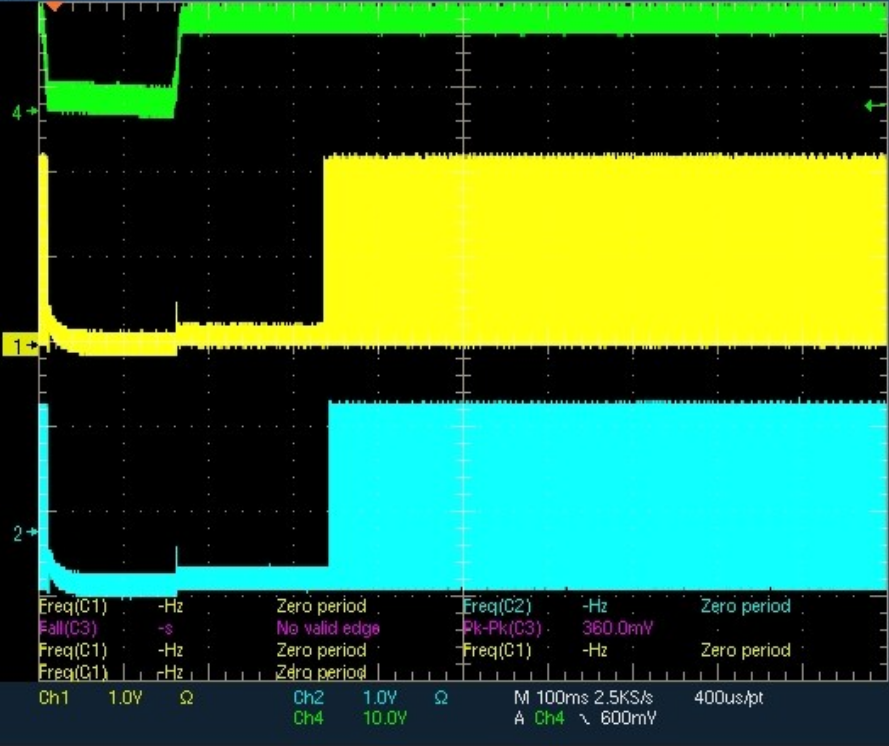
\includegraphics[width=\linewidth, trim={0 0 0 0}, clip]{fig/PowerReboot.png}
\caption{\label{fig:sadc:pwr_rbt}Reboot time of the power supply at the SADC: green line corresponds to the power supply clock, yellow and azure lines show the clock signal of the FPGA-1 and the FPGA-2 correspondingly. }
\end{figure}Thus, the data, expected to arrive from a certain ADC module, will be lost. Hence, it is important to know how many data were lost for proper data correlation later. Therefore, another irradiation experiment was done at KVI in October 2018 to determine the recovery time after the SEU case.
\begin{figure}[htb]
\includegraphics[width=\linewidth, trim={0 0 0 0}, clip]{fig/FPGAReboot.png}
\caption{\label{fig:sadc:fpga_rbt}Reboot time of the FPGA at the SADC.}
\end{figure}

Depending on the place where the SEU has occurred, the SADC board can be fully or partially reset. In case if a power supply of the SADC module suffered from irradiation, the full reboot of the board is required. The mean time of the reboot when the main SODA clock is available for the power supply is \SI{180}{\milli\second} as shown in \Reffig{fig:sadc:pwr_rbt}. Another possible scenario is damaging the firmware configuration, which was loaded to the FPGA memory. This problem can be resolved with re-configuring the FPGAs. Time, expected for this procedure, you can see in \Reffig{fig:sadc:fpga_rbt}. For one FPGA it is around \SI{150}{\milli\second} in case of its reboot. Providing the clock does not mean the immediate data production. There is latency existing between data production and the reboot time of the FPGA, what can be explained by fetching the configuration settings from the main DAQ system to the DC and further to the SADC board. This latency is shown in \Reffig{fig:sadc:data_rd}. On average, it is \SI{15}{\milli\second}.
\begin{figure}[htb]
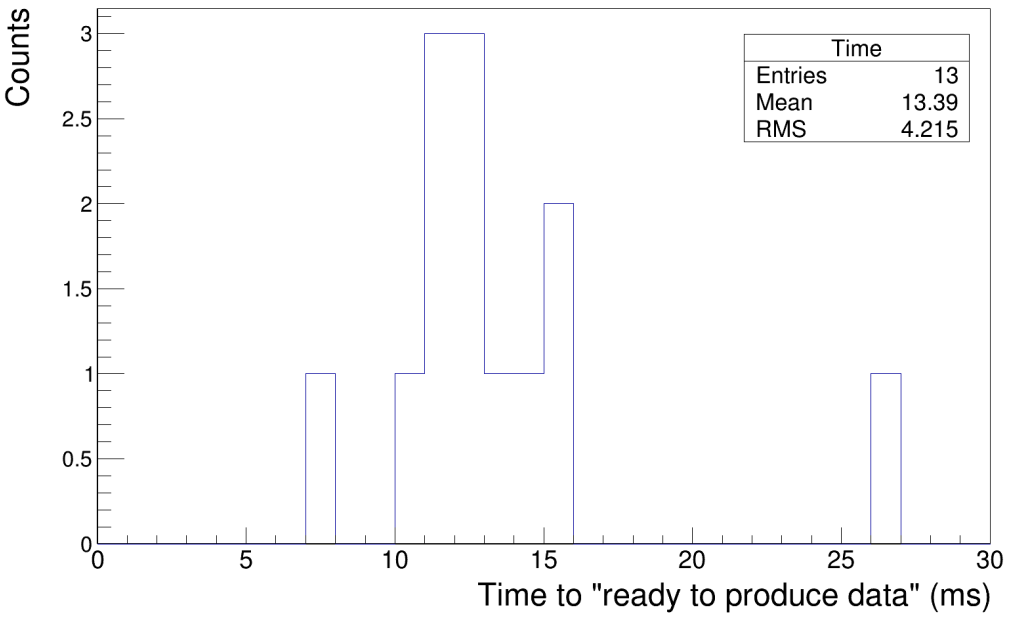
\includegraphics[width=\linewidth, trim={0 0 0 0}, clip]{fig/DataProdRd.png}
\caption{\label{fig:sadc:data_rd}Latency of the SADC before data production.}
\end{figure}
Thus, within the \SI{200}{\milli\second} the presented SADC board can back into full operation mode in both cases of the SEU occurrence, which means continuing data collection.
\section{Conclusion}
A number of prototypes of the signal digitizer for EMC for the PANDA experiment were constructed and tested. The device was found to be fulfilling the requirements concerning performance and robustness described in the Technical Design Report. The device is ready for moving to a volume production phase.

\bibliography{lit}

\end{document}